% Author: Carles Marin (Claude, Anthropic, as AI research assistant).
% Part V. What the Higgs potential cannot see: bulk matter that cannot help select a boundary
% condition. The potential is a dimension and an index. The one-loop Wilson-line potential of 6D SU(4) gauge-Higgs unification is two Schur
% specialisations of one partition, selected by the parity of the winding number; the published
% coefficients of AHMN are reproduced from representation theory alone; and the boundary-condition
% sign rides on the coset half -- Part IV's object -- so it goes blind exactly on Part IV's
% vanishing class.
% NOT the claim of an earlier draft: "the coset half is the only observable that sees charge
% conjugation". That is FALSE, retracted 2026-07-30, and contradicted in print (GATE_KKKY.md).
% English edition; the Spanish one is made once this text stops moving (paper/README.md).
% Build: pdflatex x2.  Every displayed number regenerates from ../*.py, output in ../outputs/.
\documentclass[11pt,a4paper]{article}
\usepackage[utf8]{inputenc}
\usepackage{amsmath,amssymb,amsthm}
\usepackage{booktabs}
\usepackage{longtable}   % the ledger must break across pages, or it strands one nearly blank
\usepackage{dsfont}      % \mathds{1}: amssymb has no blackboard 1 and substitutes a wrong glyph
\usepackage[table,dvipsnames]{xcolor}
\usepackage{graphicx}
\usepackage{tikz}
\usetikzlibrary{shapes.geometric,arrows.meta,positioning,fit,backgrounds,patterns,calc}
\usepackage{geometry}
\geometry{margin=2.4cm}
\usepackage[colorlinks=true,linkcolor=RoyalBlue,citecolor=BrickRed,urlcolor=RoyalBlue]{hyperref}
\usepackage{caption}
\captionsetup{font=small,labelfont=bf}
\newtheorem{theorem}{Theorem}
\newtheorem{lemma}{Lemma}
\newtheorem{corollary}{Corollary}
\newtheorem{proposition}{Proposition}
\newtheorem{observation}{Observation}
\newcommand{\ZZ}{\mathbb{Z}}
% the identity matrix: \mathbb{1} has no glyph in msbm and silently prints as \nVdash
\newcommand{\one}{\mathds{1}}
\newcommand{\su}[1]{SU(#1)}
\newcommand{\Sig}{\Sigma_\lambda}
\newcommand{\Dl}{D_\lambda}
% the thread: each section ends with the question the next one answers
\newcommand{\bridge}[1]{\par\medskip\noindent
  \textcolor{hdrblue!45}{\rule{2.2cm}{0.6pt}}\;\;\parbox[t]{0.84\textwidth}{\small\itshape
  \textcolor{hdrblue!85}{#1}}\par\medskip}

% a framed display for the equations the paper stands on -- and only those
\newsavebox{\keyeqbox}
\newenvironment{keyeq}
  {\begin{center}\setlength{\fboxsep}{9pt}\setlength{\fboxrule}{0.8pt}%
   \begin{lrbox}{\keyeqbox}\begin{minipage}{0.88\textwidth}}
  {\end{minipage}\end{lrbox}%
   \fcolorbox{hdrblue!55}{hdrblue!6}{\usebox{\keyeqbox}}\end{center}}
\definecolor{okgreen}{RGB}{0,140,54}
\definecolor{hdrblue}{RGB}{31,78,121}
\definecolor{softgrey}{RGB}{238,242,247}
\definecolor{warmred}{RGB}{178,34,34}

\title{\textbf{\Large What the Higgs Potential Cannot See:\\[2pt]
bulk matter that cannot help select a boundary condition}\\[7pt]
\large\textnormal{\itshape Winding parity is the $O(4)$ component label, so the potential is one
operator traced twice --- a \textnormal{dimension} and an \textnormal{index}; the boundary-condition
sign rides on the index alone, and goes blind on a class we classify and count in closed form}\\[8pt]
\normalsize\textnormal{Part V --- 6D $\su4$ gauge-Higgs unification: the published one-loop
coefficients of three separate papers reproduced from representation theory alone, and a selection
rule on the matter content that costs nothing to apply}}
\author{Carles Mar\'in\thanks{Independent researcher, \texttt{karlesmarin@gmail.com}.
The computations were carried out and cross-checked with Claude (Anthropic) as an AI research
assistant against a common machine-verifiable ground truth; every number in this paper regenerates
from the ancillary scripts, whose output is archived beside them.}}
\date{\today}

\begin{document}
\maketitle

\begin{abstract}
\noindent
Parts~I--IV of this series built a piece of representation theory and left its physical purpose
implicit. This paper supplies it. Part~III's own translation matrix $U_6=P_2P_0^{-1}$ has
determinant $-1$, so it does not lie in the identity component of the structure group; the
consequence is that the parity of the winding number is the $O(4)$ component label, and the entire
one-loop Wilson-line potential of the model is \emph{two Schur specialisations of one partition},
$\Sig(t)=s_\lambda(1,1,t,t^{-1})$ on the identity component and
$\Dl(t)=s_\lambda(1,-1,t,t^{-1})$ --- Part~IV's object --- on the reflection coset. The claim is
anchored to numbers we did not produce: the standard form in which this field writes its one-loop
potential, $\{A+B(-1)^{k_2}\}$, has coefficients that \emph{are} $(\Sig\pm\Dl)/2$, and the published
numbers of three separate papers --- in three groups, two dimensions and two orbifolds --- are
reproduced from representation theory with nothing fitted. The pair is one object read twice: with
$\sigma$ the orbifold parity and $g_t$ the Wilson-line element, $\sigma g_t$ is the coset alphabet,
so $\Sig=\mathrm{Tr}(g_t)$ and $\Dl=\mathrm{Tr}(\sigma g_t)$ --- a trace and a twisted trace of one
element on one space, a dimension and an index. What follows is a statement about what such a
potential can and cannot see. Each matter multiplet carries a
discrete boundary-condition sign --- in the notation Haba, Hosotani and Kawamura have used since
2004, the product $\eta=\eta_0\eta_1$ of the two signs attached to the orbifold parities --- and
that sign multiplies the coset character and nothing else. Hence:
$(\lambda,\eta)\sim(\lambda^*,\eta(-1)^{\lambda_1})$ is an observational identity --- proved, and
verified over the range swept to be the only collision there is --- and
$\eta$ is unobservable \emph{exactly} on $\mathcal Z$, Part~IV's vanishing class, whose closed-form
classification is therefore a classification of the multiplets that cannot help select a boundary
condition. The bridge to the older literature is exact and it widens the statement: for any
representation, a pair of orbifold parities sees a multiplet through exactly three characters,
$N^{(\varepsilon_0,\varepsilon_1)}=\frac14[\dim+\varepsilon_0\chi(P_0)+\varepsilon_1\chi(P_1)
+\varepsilon_0\varepsilon_1\chi(P_0P_1)]$, and $\eta$ multiplies the last one alone --- so the
theorem is not a property of one six-dimensional model but of the $[p;q,r;s]$ classification itself.
A corollary settles a difference of regime we expected to have to live with: because Part~IV's
closed form has coefficients of one sign, $\Dl(1)=0$ if and only if $\Dl\equiv0$, so the sign is
invisible at vanishing Wilson line phase --- where the 5D literature computes --- if and only if it
is invisible at every phase. Three further statements are proved or measured rather than asserted:
the blind class is counted in closed form, $\lceil(k+1)^2/2\rceil$ at $\lambda_1=2k+1$ and never for
$\lambda_1$ even --- machine-checked in Lean~4, and chained to Part~III's existing certificate so
that the count is a theorem about the bialternant determinant rather than about a predicate chosen
to be countable; the asymmetry between the two halves is traced to the frozen letters being a
complete set of roots of unity, which puts every zero of the coset character on the unit circle and
none of the identity character's there, so that the coset amplitude vanishes only at \emph{rational}
Wilson line phases; and the same test, applied to the boundary conditions themselves, shows that
$\lfloor(N+1)^2/2\rfloor$ of the $(N+1)^2$ equivalence classes admit a coset sector at all --- also
machine-checked, and for every rank rather than over a swept range, because the block pair
$(\#\{P_0{=}{+}1\},\#\{P_1{=}{-}1\})$ turns out to be a complete class invariant --- which
splits the invisibility question into one geometric case and one representation-theoretic case, only
the second of which is ours. One step past a single multiplet is then free: if the non-blind
multiplets of a matter content share one effective sign, the content is blind only if every multiplet
in it is --- so \emph{collective blindness requires sign frustration}, and the degeneracy left for
the sequel is the frustrated half of it. Scope is stated and not buried: every statement here is
about a \emph{model}, the theorem is \emph{per multiplet}, and everything that runs the machinery forwards
--- predicting a spectrum rather than excluding one --- is deliberately held over to Part~VI. \emph{Retracted before publication, and
recorded because the record is worth as much as the result:} an earlier draft of \S\ref{sec:obs}
claimed the coset half is the only observable in the model that sees charge conjugation. It is not;
charge conjugation is invisible here unconditionally, and Kawamura, Kodaira, Kojima and Yamashita
say so in print. The sign $(-1)^{\lambda_1}$ is real, but it speaks about the boundary condition.
\end{abstract}

\begin{figure}[h]
\centering
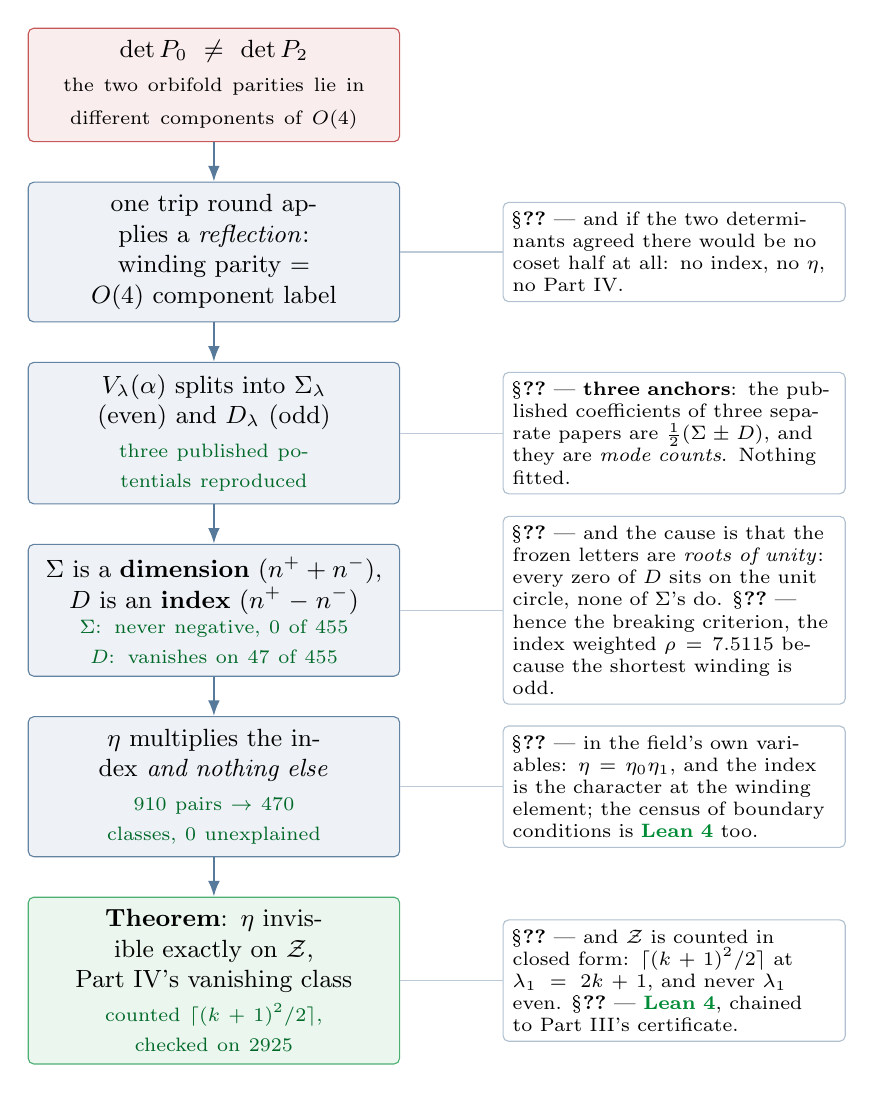
\begin{tikzpicture}[node distance=5mm, every node/.style={font=\small},
  bead/.style={draw=hdrblue!70,fill=softgrey,rounded corners=2pt,inner sep=4.5pt,
               minimum height=8mm,text width=44mm,align=center},
  root/.style={draw=warmred!75,fill=warmred!8,rounded corners=2pt,inner sep=4.5pt,
               minimum height=8mm,text width=44mm,align=center,font=\small\bfseries},
  gain/.style={draw=okgreen!70,fill=okgreen!8,rounded corners=2pt,inner sep=4.5pt,
               minimum height=8mm,text width=44mm,align=center},
  side/.style={draw=hdrblue!35,fill=white,rounded corners=2pt,inner sep=3.5pt,
               text width=41mm,align=left,font=\scriptsize},
  ar/.style={-{Latex[length=2mm]},hdrblue!75,thick}]

\node[root] (r) {$\det P_0 \neq \det P_2$\\[4pt]
  {\normalfont\scriptsize the two orbifold parities lie in\\[1pt] different components of $O(4)$}};
\node[bead,below=of r] (w) {one trip round applies a \emph{reflection}:\\
  winding parity $=$ $O(4)$ component label};
\node[bead,below=of w] (v) {$V_\lambda(\alpha)$ splits into
  $\Sigma_\lambda$ (even) and $D_\lambda$ (odd)\\[1pt]
  \scriptsize\textcolor{okgreen!75!black}{three published potentials reproduced}};
\node[bead,below=of v] (di) {$\Sigma$ is a \textbf{dimension} ($n^++n^-$),\\
  $D$ is an \textbf{index} ($n^+-n^-$)\\[1pt]
  \scriptsize\textcolor{okgreen!75!black}{$\Sigma$: never negative, $0$ of $455$\\
  $D$: vanishes on $47$ of $455$}};
\node[bead,below=of di] (eta) {$\eta$ multiplies the index \emph{and nothing else}\\[1pt]
  \scriptsize\textcolor{okgreen!75!black}{$910$ pairs $\to$ $470$ classes, $0$ unexplained}};
\node[gain,below=of eta] (thm) {\textbf{Theorem}: $\eta$ invisible exactly on
  $\mathcal Z$, Part~IV's vanishing class\\[1pt]
  \scriptsize\textcolor{okgreen!75!black}{counted $\lceil(k+1)^2/2\rceil$, checked on $2925$}};

\node[side,right=13mm of w] (s1) {\S\ref{sec:spine} --- and if the two determinants agreed there
  would be no coset half at all: no index, no $\eta$, no Part~IV.};
\node[side,right=13mm of v] (s2) {\S\ref{sec:anchor} --- \textbf{three anchors}: the published
  coefficients of three separate papers are $\tfrac12(\Sigma\pm D)$, and they are \emph{mode
  counts}. Nothing fitted.};
\node[side,right=13mm of di] (s3) {\S\ref{sec:two} --- and the cause is that the frozen letters are
  \emph{roots of unity}: every zero of $D$ sits on the unit circle, none of $\Sigma$'s do.
  \S\ref{sec:halves} --- hence the breaking criterion, the index weighted $\rho=7.5115$ because the
  shortest winding is odd.};
\node[side,right=13mm of eta] (s4) {\S\ref{sec:hhk} --- in the field's own variables:
  $\eta=\eta_0\eta_1$, and the index is the character at the winding element; the census of
  boundary conditions is \textbf{\color{okgreen}Lean 4} too.};
\node[side,right=13mm of thm] (s5) {\S\ref{sec:obs} --- and $\mathcal Z$ is counted in closed form:
  $\lceil(k+1)^2/2\rceil$ at $\lambda_1=2k+1$, and never $\lambda_1$ even.
  \S\ref{sec:lean} --- \textbf{\color{okgreen}Lean 4}, chained to Part~III's certificate.};

\draw[ar] (r)--(w); \draw[ar] (w)--(v); \draw[ar] (v)--(di);
\draw[ar] (di)--(eta); \draw[ar] (eta)--(thm);
\foreach \a/\b in {w/s1, v/s2, di/s3, eta/s4, thm/s5}
  \draw[hdrblue!30] (\a.east)--(\b.west);
\end{tikzpicture}
\caption{The chain, and it is one chain: every statement in this paper descends from the single
determinant at the top. Left, the thread; right, what each link buys and where it is done.}
\label{fig:chain}
\end{figure}

% ===================================================================
\section{The matrix with determinant $-1$}\label{sec:spine}

Part~III derived the Kaluza--Klein mode labels of $\su4$ gauge-Higgs unification on $T^2/\ZZ_2$ from
the orbifold boundary conditions, and in doing so wrote down its own translation matrix
\begin{equation}\label{eq:U6}
U_6 \;=\; P_2P_0^{-1} \;=\; \mathrm{diag}(1,1,-1,1),
\qquad \det U_6 \;=\; -1 .
\end{equation}
The determinant is printed there and was never used. It is the hinge of this paper, and it is worth
saying at once what acts on what, because every result below is a consequence of one sign.

An orbifold with two fixed points carries two parities, $P_0$ and $P_2$, and the geometry --- not a
choice --- makes the translation their product. Part~III's embedding puts them in \emph{different
components} of $O(4)$:
\begin{equation}\label{eq:root}
P_0=\mathrm{diag}(1,1,1,-1),\quad \det P_0=-1;
\qquad
P_2=\mathrm{diag}(1,1,-1,-1),\quad \det P_2=+1;
\end{equation}
so the $U_6$ of \eqref{eq:U6} has $\det U_6=\det P_2\cdot\det P_0=-1$: \emph{one trip around the
compact direction applies a
reflection.} That is the acting object, and what it acts on is the parity grading of the matter
multiplet.

\emph{Two things have to be said about that determinant before anything is built on it, because both
are what a reader should suspect first.}

\emph{It is not a convention.} The parities act on the gauge field by conjugation, and conjugation
does not see an overall phase: $P$ and $zP$ act identically. But the orbifold condition is
$P^2=\one$ --- stated in exactly that form in \cite{HHK}, their eq.~(2.4),
$T[P_0]^2=T[P_1]^2=I$, and in \cite{KKKY} --- and it forces $z^2=1$, hence $z=\pm1$, hence
$\det(zP)=z^4\det P=\det P$. The phase that would flip a determinant in four dimensions is
$z=e^{i\pi/4}$, and it gives $(zP)^2=i\,\one$, which is not a parity at all. So $\det P$ is
pinned by the orbifold condition and is not ours to choose. \emph{On matter} the phase does act, and
that is a different statement: it is precisely the boundary sign $\eta$ of \S\ref{sec:obs}. (A setup
in which $P^2$ is only required to lie in the centre would allow $z^8=1$ and hence $z^4=\pm1$, and
the determinant would no longer be fixed; that is not the condition used here or in the sources.)

\emph{And it is a statement about the matrix, not about the gauge algebra.} Conjugation by any
unitary is an \emph{inner} automorphism of $\mathfrak{su}(4)$, since $U=e^{i\theta}V$ with
$V\in\su4$ conjugates identically; nothing here claims otherwise. What lies in the non-identity
component of $O(4)$ is the matrix $P_0$ itself --- real, orthogonal, $\det=-1$ --- and that is what
the character needs, because $s_\lambda$ is being evaluated at its eigenvalue alphabet. The
determinant enters through the alphabet, not through the automorphism.

The control on \eqref{eq:root} is one line and it could have gone the other way. Had the two parities shared a
determinant --- either both $+1$ or both $-1$ --- the translation would lie in the identity
component, every winding with it, and there would be no coset half at all: no index, no
boundary-condition sign to be invisible, no vanishing class, and no Part~IV. The entire series exists
because $\det P_0\neq\det P_2$.

Everything below is that fact propagating, and Figure~\ref{fig:chain} is the whole descent on one
page: the winding parity becomes the component label
(\S\ref{sec:spine}); the potential splits into a dimension and an index (\S\ref{sec:two}); the
shortest winding is the reflection itself, which is why the index outweighs the dimension
(\S\ref{sec:halves}); the reflection is not in $\su4$, so acting with it on a multiplet requires
choosing an extension, and that choice is $\eta$ (\S\ref{sec:obs}); and $\eta$ is invisible exactly
where the reflection acts with balanced multiplicities (Corollary~\ref{cor:balance}).

The $(k_1,k_2)$ winding amplitude of the one-loop potential is the character of the matter multiplet
at the holonomy $\exp(i\pi\theta T)\,U_6^{\,k_2}$, with $T=\mathrm{diag}(0,1,0,-1)$ and
$\theta=k_1\alpha_1+k_2\alpha_2$. Writing $t=e^{i\pi\theta}$, the eigenvalue alphabet of that
holonomy is
\begin{keyeq}
\begin{equation}\label{eq:alphabets}
\begin{array}{llll}
k_2 \text{ even:} & (\,1,\;1,\;t,\;t^{-1}\,), & \det=+1, & \text{identity component},\\[2pt]
k_2 \text{ odd:} & (\,1,-1,\;t,\;t^{-1}\,), & \det=-1, & \text{reflection coset.}
\end{array}
\end{equation}
\end{keyeq}
So the \emph{parity of the winding number is the $O(4)$ component label}. Part~IV opened by saying
that its alphabet $(1,-1,t,t^{-1})$ ``arrived from physics\dots not from a search of the
combinatorial literature'', and could not say why that alphabet and not another. Equation
\eqref{eq:alphabets} is why: it is the generic semisimple element of the non-identity component, and
the physics reaches it because $U_6$ is not in the identity component. [Verified: $18$ of $18$ exact
matches of the split against Part~III's published histograms, \texttt{potential\_split.sage}.]

Two scope statements belong here rather than at the end. The construction is $T^2/\ZZ_2$ with
$U_5=\one$; on $T^2/\ZZ_4$ the winding sum is a two-element trace
$\mathrm{Tr}\,[W_1^{w_1}W_2^{w_2}]$ and is not a single-holonomy character, so nothing below applies
there without redoing it. And the grading of the potential by the centre charge, which one might
think is the content of \eqref{eq:alphabets}, is classical twice over --- Davies and
McLachlan~\cite{DM}, already cited in Part~III, and Roberge--Weiss periodicity~\cite{RW}; the
modern statements of the same grading are in \"Unsal--Yaffe and Argyres--\"Unsal~\cite{ArgyresUnsal}
and Ogilvie~\cite{Ogilvie}. What is offered here is the identification of the two components, not the
grading.

The setting itself is old and crowded, which is why every section below states what it inherits.
Unifying the Higgs with the extra-dimensional components of a gauge field goes back to
Manton~\cite{Manton}; that the resulting Wilson-line phases are dynamical, and break the symmetry by
radiative corrections rather than by hand, is the Hosotani mechanism~\cite{Hosotani}; the orbifold
construction that makes four-dimensional chiral fermions possible and splits the Higgs multiplet is
due to Kawamura~\cite{Kawamura} and Hall--Nomura~\cite{HallNomura}, with the supersymmetry-breaking
twist of Scherk--Schwarz~\cite{SS}. The closest five-dimensional computation to the object of this
paper --- the one-loop potential as a function of the Wilson line phase within one equivalence class
--- is Haba, Harada, Hosotani and Kawamura~\cite{HHHK}.

\bridge{One determinant, and the winding sum splits in two. Into what, exactly --- and are the two
pieces related, or merely adjacent?}

% ===================================================================
\section{The potential is two Schur specialisations}\label{sec:two}

\subsection*{What the Higgs is in this model}

Nothing below is about a scalar field added to a Lagrangian. In gauge-Higgs unification the Higgs
\emph{is} the Wilson-line phase: the extra-dimensional components $A_5,A_6$ of the $\su4$ gauge field
on $T^2/\ZZ_2$ furnish two four-dimensional doublets, the tree-level potential is
$\mathrm{Tr}\,[A_5,A_6]^2$ and is flat along the Wilson line, and the degeneracy is lifted only at one
loop, by the Hosotani mechanism~\cite{Hosotani}. The vacuum expectation value of the Higgs is
therefore a \emph{phase} $\alpha$, chosen by the minimum of the one-loop potential; the Higgs mass is
the curvature of that potential at the minimum; and the couplings $\kappa_V$ follow from the same
function. That is the entire electroweak sector of the model, and it is a sum over windings of the
compact directions.

Writing $W_k$ for the (representation-independent) winding weight and $\theta_k=k_1\alpha_1+k_2\alpha_2$,
the one-loop potential of a multiplet $\lambda$ is exactly

\begin{keyeq}
\begin{equation}\label{eq:V}
V_\lambda(\alpha)\;=\;\sum_{k\neq0}W_k\cdot
\begin{cases}
\Sig\big(e^{i\pi\theta_k}\big), & k_2 \text{ even} \quad\text{(identity component)},\\[3pt]
\Dl\big(e^{i\pi\theta_k}\big), & k_2 \text{ odd} \quad\;\;\text{(reflection coset)} .
\end{cases}
\end{equation}
\end{keyeq}

\noindent [Verified on all nine representations of the model's library.] Everything physical in this
paper is read off \eqref{eq:V}: the vacuum is its minimum, the Higgs mass its curvature, and the
question of \S\ref{sec:obs} --- what a boundary condition can do that anybody could measure --- is
the question of what can change \eqref{eq:V}.

\subsection*{The two functions, and why only one of them can vanish}

From \eqref{eq:alphabets}, every winding contributes through one of exactly two functions of the
\emph{same} partition $\lambda$ labelling the multiplet:
\begin{equation}\label{eq:SigD}
\Sig(t) \;=\; s_\lambda(1,\;1,\;t,\;t^{-1}),
\qquad
\Dl(t) \;=\; s_\lambda(1,-1,\;t,\;t^{-1}).
\end{equation}
Part~IV computed $\Dl$ and gave a closed form for it: up to a sign it is a product of exactly
three $\su2$ characters read off the $2$-quotient of $\lambda$, or identically zero, with no
hypothesis on the shape of $\lambda$. \emph{Part~IV states that identity as verified and not
proved} --- checked there exhaustively, by two independent implementations, over the ranges it
declares, with no mismatch --- and every statement in this paper that rests on it inherits that
standing exactly; \S\ref{sec:scope} says which ones. The identity sits between two factorisation
programmes and belongs to neither: the reciprocal-pair line of Ciucu--Krattenthaler~\cite{CK} and
Ayyer--Behrend~\cite{AB}, and the twining-character line of Jantzen~\cite{Jantzen} and
Kumar--Lusztig--Prasad~\cite{KLP}, whose folding identity is the mechanism behind it. In the
exponential expansion this makes the coset half a
\emph{box}:
\begin{equation}\label{eq:box}
V_{\mathrm{odd}}(\alpha) \;=\; \zeta \sum_{c\,\in\,\mathrm{Box}(a_1,a_2,a_3)} G\big(m(c)\,\alpha\big),
\qquad m(c)=\textstyle\sum_i a_i - 2\sum_i c_i ,
\end{equation}
where $\mathrm{Box}(a_1,a_2,a_3)=\{c\in\ZZ^3 : 0\le c_i\le a_i\}$ and $(a_1,a_2,a_3)$ are the sides
read off the $2$-quotient, so that $m(c)$ runs over the winding charges of the multiplet with the
right multiplicities. The function $G$ in \eqref{eq:box} is one and the same for every
representation: the multiplet
enters only as a
multiset of integers read off its Young diagram. That multiset is the list which
AHMN~\cite{AHMN} (their eq.~(3.25)) and Kawamura \emph{et al.}~\cite{KKKY} (their eqs.~(5.22)--(5.28))
assemble by hand from the Kaluza--Klein spectrum. The curvature of that half --- the contribution to
the Higgs mass --- is its second moment,
$\partial^2_{\alpha_2}V_{\mathrm{odd}}=\zeta\sum_a m(a)^2G''(m\alpha)$ [verified $9/9$ at a generic
point, \texttt{box\_potential.py}], and that second moment is the sum of the three $\su2$ Casimirs
of the box [verified $2197/2197$ over all boxes with sides $\le12$, \texttt{verify\_formulas.py}].

\emph{Notation, and it is a collision we have to disarm.} Part~IV writes the sides of the box as
$(p,q,r)$. The five-dimensional literature we bridge to in \S\ref{sec:hhk} writes the block sizes of
the orbifold parity matrices as $[p;q,r;s]$, and has done so since 2004. The two triples are
unrelated and both are load-bearing here. Throughout this paper the box of Part~IV is written
$(a_1,a_2,a_3)$ and $[p;q,r;s]$ keeps its established meaning.

\begin{figure}[t]
\centering
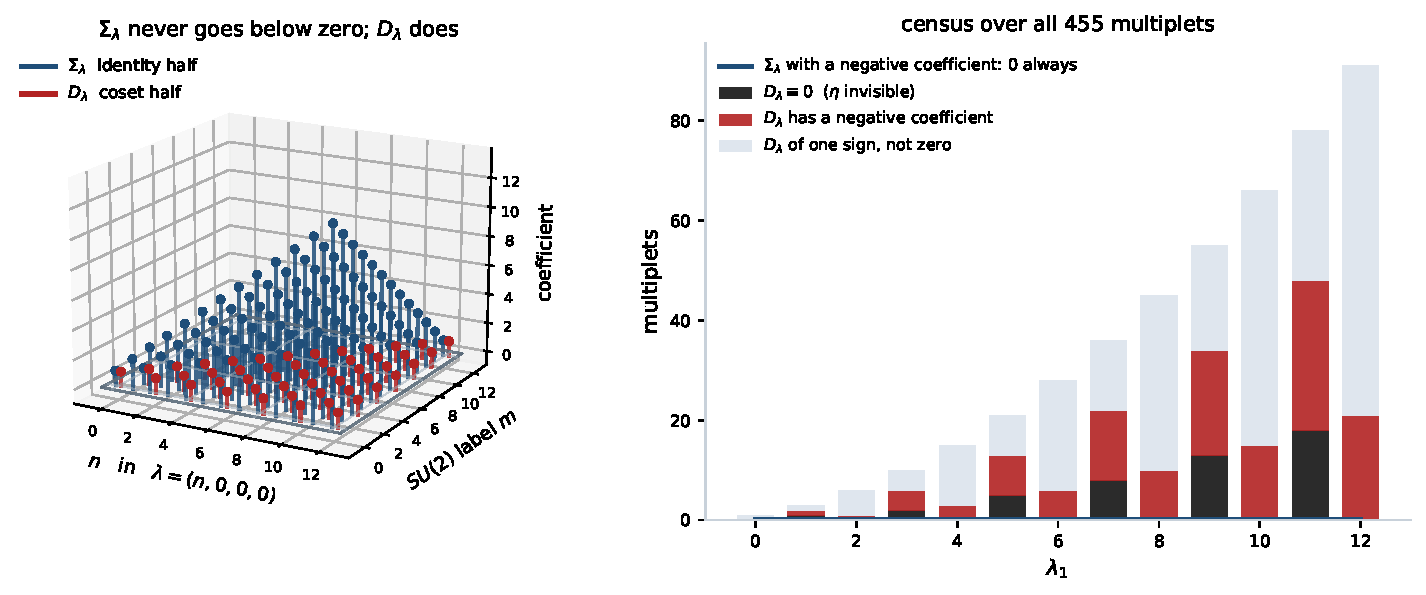
\includegraphics[width=\textwidth]{fig_positivity.pdf}
\caption{The asymmetry of \eqref{eq:dimindex}, measured. \textbf{Left:} the two halves expanded in
$SU(2)$ characters over the symmetric family $\lambda=(n,0,0,0)$, which contains AHMN's
$\mathbf{35}=(4,0,0,0)$. Each stem is one coefficient, and the outlined frame is the zero level. Every
blue stem stands above it, because the identity half's coefficients are dimensions $n^+_m+n^-_m$;
the red ones hang below it, because the coset half's are indices $n^+_m-n^-_m$. \textbf{Right:} the census over all $455$ multiplets in
range, by $\lambda_1$ and disjointly: those with $D_\lambda\equiv0$ (the blind class, $47$), those
whose $D_\lambda$ has a coefficient of each sign ($134$), and the rest. The flat line is the count of
multiplets whose $\Sigma_\lambda$ has a negative coefficient: it is $0$ at every $\lambda_1$, and by
\eqref{eq:dimindex} it must be. Generated by \texttt{make\_figure\_positivity.py}.}
\label{fig:posit}
\end{figure}

\subsection*{Why one half factors and the other cannot}

That $\Dl$ always factors and $\Sig$ never does is not a difference of degree, and the cause is not
that one alphabet has an extra letter. It is that $\{1,-1\}$ is the complete set of square roots of
unity and $\{1,1\}$ is not. Attaching one free reciprocal pair $\{z,z^{-1}\}$ to a frozen block $F$
and asking, by Kronecker's criterion, whether every zero of $s_\lambda$ lies on the unit circle ---
equivalently whether the character is a monomial times a product of cyclotomic polynomials:

\begin{center}\small
\rowcolors{2}{softgrey}{white}
\begin{tabular}{lrrrl}
\toprule
\rowcolor{hdrblue!14}frozen block $F$ & non-zero & all zeros on $|z|=1$ & share & worst failure\\
\midrule
$\mu_2=\{1,-1\}$ & $212$ & $212$ & $100\%$ & ---\\
$\{1,1\}$ & $241$ & $16$ & $6.6\%$ & $1.62$\\
$\mu_3$ & $124$ & $124$ & $100\%$ & ---\\
$\{1,1,1\}$ & $150$ & $3$ & $2.0\%$ & $2.73$\\
$\mu_4$ & $86$ & $86$ & $100\%$ & ---\\
$\{1,1,1,1\}$ & $125$ & $2$ & $1.6\%$ & $3.79$\\
\bottomrule
\end{tabular}
\end{center}

\noindent \emph{Only the second column of that table is ours, and the distinction matters.} That a
root-of-unity block forces a factorisation is classical and has a long line: Littlewood and
Richardson showed the Verschiebung action on $s_\lambda$ vanishes when the $t$-core is non-empty and
otherwise factors over the $t$-quotient; Lecouvey~\cite{Lecouvey} and Ayyer--Kumari~\cite{AK} did the
symplectic and orthogonal cases, characterising non-vanishing by $z$-asymmetric partitions through a
study of beta sets; Albion~\cite{Albion} embeds all of them in one family. \emph{Our} alphabet ---
all $t$-th roots of unity together with one free reciprocal pair --- is in none of them: that line's
alphabets carry a free variable in every letter, and ours carries exactly one. So the $100\%$ rows
are measured here rather than read off a published theorem, and at $t=2$ they are the zero locus of
Part~IV's closed form, with its standing.

What is new here is the \textbf{control}: nobody had a reason to run the repeated-letter blocks,
because there is no theorem there to prove. We had a reason --- $\{1,1\}$ is the identity half of a
Higgs potential --- and the answer is that they factor essentially never, and fail grossly. A zero
off the circle by $1.62$ in modulus is not a numerical artefact, whereas the
root-of-unity blocks fail only at a tolerance of $10^{-7}$ with deviations of order $5\times10^{-6}$
and pass at $10^{-4}$ [\texttt{why\_one\_factors.py}].

\emph{And the division of labour is not the one this series assumed.} Four papers went to $\Dl$
because it has zeros to classify and $\Sig$ has none, and the sentence above says why. But having no
zeros is not the same as carrying no information, and it turns out to be the other way round:
$\Sig$ \emph{alone} determines the multiplet up to conjugation --- its fibres over $969$ multiplets
are exactly the orbits $\{\lambda,\lambda^*\}$, with the singletons exactly the self-conjugate ones
(\S\ref{sec:scope}). So the even-winding half of the potential carries the \emph{identity} of the
matter, and the odd-winding half carries the \emph{boundary condition}. The half nobody mined is the
one that says what the matter is.

Figure~\ref{fig:zeros} is the same statement
counted zero by zero instead of polynomial by polynomial.

Two consequences worth separating. \emph{Mathematically}, ``factors into three $SU(2)$ characters''
is the right statement only at $t=2$: at $t=3$ the pieces are cyclotomic and are \emph{not} $SU(2)$
characters --- $\lambda=(2,1,0,0,0)$ gives $z-1+z^{-1}$, the sixth cyclotomic polynomial. The uniform
statement across $t$ is the location of the zeros. \emph{Physically}, and this is the reading:
\emph{the coset amplitude of a multiplet vanishes only at rational Wilson line phases}, because its
zeros are roots of unity in $z=e^{i\pi\theta}$; the identity amplitude has its zeros off the physical
line entirely. One half is built to vanish at special points of the Wilson line and the other is not.

\begin{figure}[t]
\centering
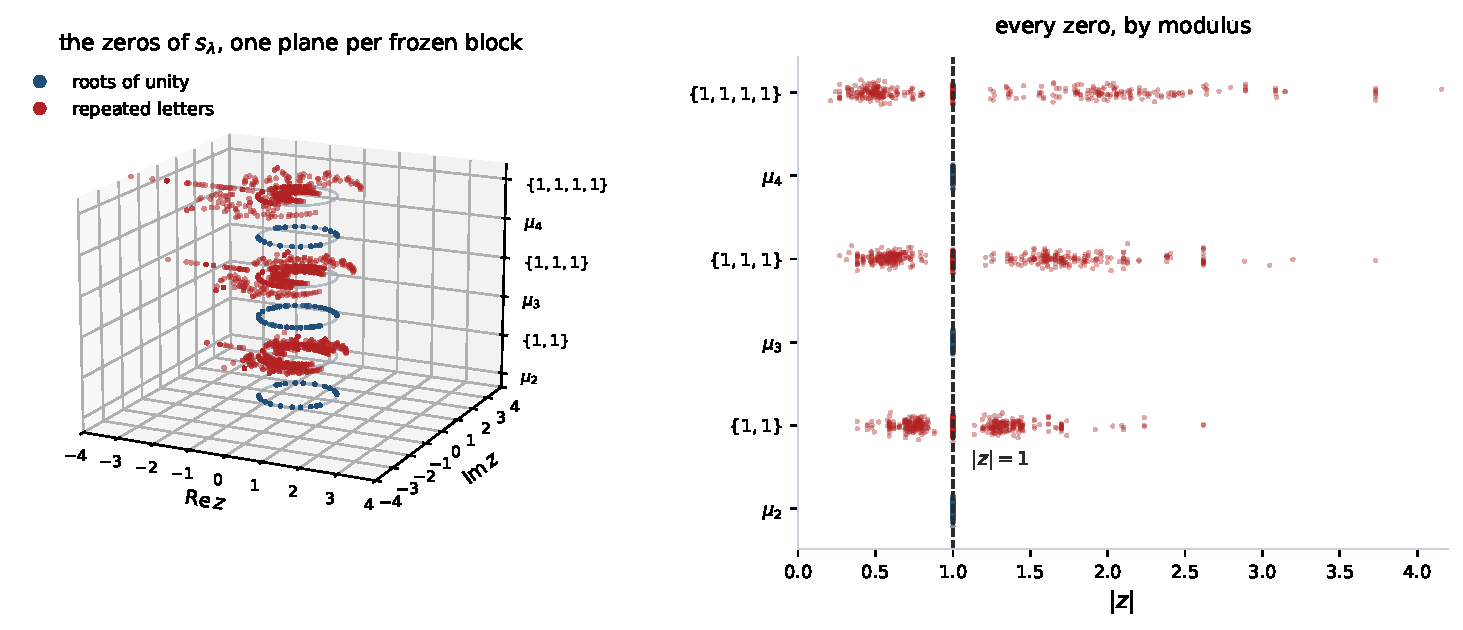
\includegraphics[width=\textwidth]{fig_zeros.pdf}
\caption{The same dichotomy at the level of individual zeros rather than of percentages.
\textbf{Left:} the complex $z$-plane stacked once per frozen block, with the unit circle drawn on
each layer. Every zero of every $s_\lambda$ built on a root-of-unity block lies \emph{on} its circle;
every repeated-letter block scatters them off it. \textbf{Right:} the same points by modulus. The
root-of-unity blocks are a single spike at exactly $1$; the others spread to $|z|=2.618$, $3.732$ and
$4.791$. Counting zeros rather than polynomials: $618$, $408$ and $218$ zeros for $\mu_2,\mu_3,\mu_4$,
all at $|z|=1$ to $10^{-4}$; and $51.6\%$, $37.5\%$, $22.5\%$ for $\{1,1\}$, $\{1,1,1\}$,
$\{1,1,1,1\}$. \emph{The coset half of the potential is built to vanish at rational Wilson line
phases; the identity half is not.} Generated by \texttt{make\_figure\_zeros.py}.}
\label{fig:zeros}
\end{figure}

\subsection*{The two halves are one operator, traced twice}

Before the reading, the identity that makes it exact rather than evocative. Let
$\sigma=\mathrm{diag}(1,-1,1,1)$ --- Part~III's orbifold parity --- and let
$g_t=\mathrm{diag}(1,1,t,t^{-1})$ be the Wilson-line element. Then
$\sigma\,g_t=\mathrm{diag}(1,-1,t,t^{-1})$: \emph{the coset alphabet is $\sigma$ times the identity
alphabet}, letter by letter. So the two halves of \eqref{eq:V} are

\begin{keyeq}
\begin{equation}\label{eq:tracepair}
\Sig(t)\;=\;\mathrm{Tr}_{V_\lambda}\big(g_t\big),
\qquad
\Dl(t)\;=\;\mathrm{Tr}_{V_\lambda}\big(\sigma\,g_t\big),
\end{equation}
\end{keyeq}

\noindent the \emph{trace} and the \emph{$\sigma$-twisted trace} of the same group element on the
same space [verified: the alphabet identity, and $\tfrac12(\Sigma\pm D)$ non-negative integers at
every charge on all multiplets in range, $287$ checks, $0$ failures,
\texttt{verify\_formulas.py}]. Everything in this paper is a consequence of reading one operator
twice. A trace is a dimension and cannot vanish; a twisted trace is an index and can. The boundary
sign multiplies the twisted one and nothing else. The blind class is where the grading balances. And
the standard form in which this field writes its one-loop potential, $\{A+B(-1)^{k_2}\}$, is that
same pair: $A$ and $B$ are the $\sigma$-even and $\sigma$-odd mode counts, and $A\pm B$ are the trace
and the twisted trace. Three separate papers~\cite{AHMN,HY,HHHK} write the twist that exchanges them
in three vocabularies --- an antiperiodic boundary condition, $Qa\mapsto Qa+\tfrac12$, and
$a\mapsto a-\beta$ --- and none names it as one operation.

\emph{The limit of that language, stated so it is not read for more than it is.} ``Twisted trace''
here is exact bookkeeping and not an index theorem: what classifies the vanishing locus is
combinatorics of the $2$-quotient and the beta-set (Part~IV, and the line from Littlewood--Richardson
through \cite{Lecouvey,AK,Albion}), not an analytic index. We claim the identity \eqref{eq:tracepair}
and the consequences drawn from it, and nothing index-theoretic.

\subsection*{The root of the asymmetry: a dimension and an index}

The two halves behave differently, and the reason is not a metaphor about cancellation. Let
$\sigma=\mathrm{diag}(1,-1,1,1)$ --- Part~III's orbifold parity --- and let $SU(2)_{34}$ be the
subgroup acting on the last two coordinates, whose torus is exactly
$\mathrm{diag}(1,1,t,t^{-1})$. \emph{They commute}, because they act on complementary coordinates. So
$V_\lambda$ decomposes under $SU(2)_{34}\times\langle\sigma\rangle$, and writing $n^\pm_m$ for the
multiplicity of the spin-$\tfrac m2$ representation inside the $\sigma=\pm1$ eigenspace, the
expansions of the two halves in $SU(2)$ characters $\chi_m$ are

\begin{keyeq}
\begin{equation}\label{eq:dimindex}
\Sig \;=\; \sum_m \big(n^+_m+n^-_m\big)\,\chi_m ,
\qquad
\Dl \;=\; \sum_m \big(n^+_m-n^-_m\big)\,\chi_m .
\end{equation}
\end{keyeq}

\noindent The first coefficient is a \emph{dimension} and the second is an \emph{index}. That is the
whole asymmetry, and it is not a choice of language: it is checkable, because it asserts that
$\tfrac12(\Sigma_\chi\pm D_\chi)$ are non-negative integers. [Verified on all $455$ multiplets in
range: $0$ non-integers, $0$ negative. And measured: $\Sig$ has a negative $SU(2)$ coefficient in
$0$ of $455$, while $\Dl$ has one in $134$ --- Figure~\ref{fig:posit}.]

Two things follow, and the second is the one this paper needed.

\begin{corollary}\label{cor:balance}
$\lambda\in\mathcal Z$ if and only if $n^+_m=n^-_m$ for \emph{every} $m$: the vanishing class is
exactly the multiplets in which every $SU(2)$ level is parity-balanced.
\end{corollary}

\noindent [Verified: $47$ level-balanced, $47$ in $\mathcal Z$, $0$ disagreements.] This refines
Part~IV, which shows that the \emph{total} parity index $n_+-n_-$ vanishes on $\mathcal Z$. Together
with Corollary~\ref{cor:regime} the chain closes: a single number vanishing --- one conserved trace
at one fixed point --- forces balance at every level of the decomposition.

And it gives $\eta$ its meaning in one sentence. The boundary sign multiplies the coset half, that is
the index; a multiplet whose levels are balanced has index zero at every level, so there is nothing
for the sign to multiply. \emph{Invisibility of the boundary condition is exact parity balance of the
matter multiplet.}

\medskip
The same statement in the older language: on weights, the identity component carries
$m_\mu+m_{\mu^*}$, which is non-negative so that nothing can cancel, and the coset carries
$m_\mu-m_{\mu^*}$, which is signed so that cancellation is possible. Hence:

\begin{center}
\fcolorbox{warmred!55}{warmred!5}{\begin{minipage}{0.88\textwidth}
\emph{Even-winding contributions to the Higgs potential can never vanish. Odd-winding ones can, and
do, for a set of representations Part~IV classifies in closed form.}
\end{minipage}}
\end{center}

\noindent Part~IV's vanishing criterion therefore has a physical reading: it says \emph{which
multiplets contribute nothing to the odd-winding part of the Higgs potential}. Everything in
\S\ref{sec:obs} is a consequence of that one sentence, because the boundary sign lives on exactly
that part.

The identity half does not collapse to a single box, and the contrast is sharper than a count
suggests. Over the $359$ partitions with at most four rows and $|\lambda|\le16$, exactly $5$ have
$\Sig$ equal to a product of at most three $\su2$ characters --- and those five are $(n,n,n,n)$ for
$n=0,\dots,4$, five partition-representatives of the \emph{same} $\su4$ irreducible, the singlet,
each with $\Sig\equiv1$. \emph{Non-trivial factorisations: none.} Where $\Dl$ always factors, $\Sig$
never does [\texttt{verify\_formulas.py}, ported from the original Sage check]. In the same block
basis, however, it is an explicit \emph{positive superposition} of the same boxes,
\begin{equation}\label{eq:evenstack}
s_\lambda(1,1,t,t^{-1}) \;=\; \sum_{0\le q\le p\le\lambda_1}(p-q+1)\,B(p,q),
\qquad B(p,q)=\chi_{m_1}\chi_{m_2}\chi_{m_3},
\end{equation}
with $m_1=\lambda_1-\max(p,\lambda_2)$, $m_2=\min(p,\lambda_2)-\max(q,\lambda_3)$,
$m_3=\min(q,\lambda_3)-\lambda_4$, and a term dropped whenever any $m_i<0$
[verified $286/286$ in exact integer arithmetic, \texttt{verify\_formulas.py}], under the weight
$s_\nu(1,1)=p-q+1$ where the coset half carries the
alternating $s_\nu(1,-1)$.

\emph{The summation range in \eqref{eq:evenstack} is not a choice, and it is worth saying so because
an unstated range is a hidden hypothesis.} Since $\max(a,b)+\min(a,b)=a+b$, the three block indices
satisfy
\begin{equation}\label{eq:degid}
m_1+m_2+m_3 \;=\; (\lambda_1-\lambda_4)-|p-\lambda_2|-|q-\lambda_3|
\end{equation}
[$0$ failures in $674\,245$ pairs]. By \eqref{eq:degid} the summand is supported exactly where
$\lambda_1\ge\max(p,\lambda_2)\ge\min(p,\lambda_2)\ge\max(q,\lambda_3)\ge\min(q,\lambda_3)\ge\lambda_4$
--- an interlacing chain whose first, third and fifth gaps are $m_1,m_2,m_3$. That support is finite
and the condition $m_i\ge0$ enforces it by itself: summing over $0\le p,q\le\lambda_1$, over
$[-15,\lambda_1{+}15]^2$ and over $[-40,\lambda_1{+}40]^2$ gives the same answer, $0$ failures of
$60$ multiplets each; and of the $4104$ pairs with all three $m_i\ge0$ that occur across those three
boxes, exactly $0$ have $q>p$, so even $q\le p$ is implied rather than imposed. There is no range
constant to get right.

The \emph{positivity} of that expansion is not a finding and we do not
present it as one: $\mathrm{diag}(1,1,t,t^{-1})$ is the torus of an $SU(2)$ subgroup, so
$\Sig$ is a restriction of $V_\lambda$ to that subgroup and its multiplicities are non-negative for
the reason all multiplicities are. What is ours is the explicit weight $p-q+1$ and the block indices
it runs over. So the whole one-loop potential, both halves, is a stack of boxes built
from the one universal $G$; the coset half collapses to a single box because its weights alternate,
and the identity half does not because its weights are positive.

This is worth stating as a physical claim and not only as a symmetric-function identity, because it
is the operational content of the whole construction:

\begin{center}
\fcolorbox{okgreen!55}{okgreen!5}{\begin{minipage}{0.88\textwidth}
\emph{For any multiplet, the entire one-loop Higgs potential \eqref{eq:V} --- both halves --- is a
positive-integer-weighted sum of one universal function evaluated at integer charges read off the
Young diagram, the coset half carrying one global sign $\zeta$ in front of it. No Kaluza--Klein
spectrum has to be enumerated.}
\end{minipage}}
\end{center}

\noindent \emph{The claim has to be narrowed, and here is the narrowing.} A general one-loop
potential for this kind of model is not new: Haba and Yamashita~\cite{HY} give one for 5D $\su N$ on
$S^1/\ZZ_2$ in 2004, with explicit formulas for the adjoint, the fundamental and the (anti)symmetric
tensors and a method they state extends to higher representations. What is not in their paper, nor
in \cite{AHMN} whose eq.~(3.25) and \cite{KKKY} whose eqs.~(5.22)--(5.28) are lists assembled
\emph{per representation} from the mode expansion, is a formula \emph{closed in $\lambda$}: one
universal function whose integer charges are read off the Young diagram of \emph{any} irreducible,
with no decomposition performed representation by representation. That, and only that, is the claim
here. The consequence is that the vacuum $\alpha_{\min}$,
the curvature at it, and $\kappa_V$ become computable for \emph{arbitrary} matter content rather than
for the handful whose spectra someone has written out. What one then \emph{does} with that --- run it
forwards to predict a spectrum --- is Part~VI's business, not this paper's.

Two honest limits on that claim, stated here and not later. The identity stack may still have a
shorter description; we do not have one. And a closed form for the \emph{potential} is not yet a
closed form for the \emph{Higgs mass}: the mass is the curvature at the true minimum, and only the
curvature at the origin is available in closed form so far. Mining the identity half for the leading
behaviour of $m_h$ is open, and it is the piece of this series we have looked at least.

\bridge{Three pairs have now appeared and all three transform the same way: the two $O(4)$
components, the two eigenspaces of the associate involution, and the two orbifold mode parities.
Three coincidences, or one object seen three times?}

% ===================================================================
\section{One $\ZZ_2$, seen three times}\label{sec:onez2}

Before the anchor, it is worth saying what the objects of \S\ref{sec:two} have in common, because
they are not three coincidences. Every formula in this paper is the same $\ZZ_2$ Fourier transform
--- $\{f_+,f_-\}\mapsto\{f_++f_-,\,f_+-f_-\}$ --- read at three different levels, and the content of
the paper is that the three agree.

\begin{center}\small
\rowcolors{2}{softgrey}{white}
\begin{tabular}{p{3.2cm} p{5.3cm} p{6.3cm}}
\toprule
\rowcolor{hdrblue!14}\textbf{level} & \textbf{the $\ZZ_2$} & \textbf{what the transform gives}\\
\midrule
the group & $\pi_0(O(4))$: identity component vs.\ reflection coset & $\Sig$ and $\Dl$, selected by
the parity of the winding\\
the multiplet & $\sigma=\mathrm{diag}(1,-1,1,1)$ acting on $V_\lambda$ & $\Sigma_\chi=n^++n^-$ (a
dimension) and $D_\chi=n^+-n^-$ (an index), \eqref{eq:dimindex}\\
the spectrum & the orbifold parity of a Kaluza--Klein mode & $A=\tfrac12(\Sigma+D)$ and
$B=\tfrac12(\Sigma-D)$, the published coefficients of \S\ref{sec:anchor}\\
\bottomrule
\end{tabular}
\end{center}

\noindent The third row is the one that turns the anchor from an agreement of two lists into a
statement with a mechanism. AHMN obtain their $A$ and $B$ by counting Kaluza--Klein modes of each
orbifold parity at each charge. Our claim is that $\Sig$ and $\Dl$ are the \emph{generating
functions} of exactly that count, so $A$ and $B$ are not fitting constants: they are mode numbers.
That is a falsifiable arithmetic statement --- $\tfrac12(\Sigma\pm D)$ must be \emph{non-negative
integers} at every charge, for every multiplet --- and it holds:

\begin{center}\small
\rowcolors{2}{softgrey}{white}
\begin{tabular}{lr}
\toprule
\rowcolor{hdrblue!14}\textbf{check over the $455$ multiplets in range} & \textbf{failures}\\
\midrule
$A=\tfrac12(\Sigma+D)$ a non-negative integer at every charge & $0$\\
$B=\tfrac12(\Sigma-D)$ a non-negative integer at every charge & $0$\\
$\tfrac12(\Sigma_\chi\pm D_\chi)$ non-negative integers (the multiplet level) & $0$\\
\rowcolor{okgreen!14}$\Dl$ with $SU(2)$ coefficients of \textbf{both} signs & $\mathbf{0}$\\
\bottomrule
\end{tabular}
\end{center}

The last row is a consequence of Part~IV and it is the sharpest of the four. Part~IV's closed form
gives $\Dl=\zeta\,\chi_{a_1}\chi_{a_2}\chi_{a_3}$ or $0$; a product of $SU(2)$ characters has non-negative
Clebsch--Gordan multiplicities; therefore

\begin{keyeq}
\begin{equation}\label{eq:onesign}
n^+_m-n^-_m \;=\; \zeta\cdot c_m,\qquad c_m\ge0\ \text{for every } m .
\end{equation}
\end{keyeq}

\noindent \emph{The parity imbalance of a multiplet points the same way at every $SU(2)$ level}, and
$\zeta$ --- which Part~IV identified as the sign of the total parity index --- is that single
direction. Corollary~\ref{cor:balance} is then immediate rather than surprising: by \eqref{eq:onesign} a sum of
terms of one sign vanishes only if every term does, so a vanishing total index forces balance level
by level.
Corollary~\ref{cor:regime} is the same argument in the other basis.

\bridge{If the third row of that table is right, then somebody else's published coefficients --- got
by counting modes, not by any of this --- have to \emph{be} our $\tfrac12(\Sigma\pm D)$. That is a
claim about numbers we did not produce, and it is the next thing to check.}

% ===================================================================
\section{Three anchors: published potentials, reproduced}\label{sec:anchor}

A structural claim of this kind is worth nothing until it reproduces numbers someone else printed. One such agreement is a coincidence one cannot rule out, so there are three, chosen to share as little as possible.
Akamatsu, Hirose, Maru and Nago~\cite{AHMN} compute the one-loop potential of this model and write
it with coefficients of the form $\{A+B(-1)^{k_2}\}$. Under \eqref{eq:alphabets} that form is forced,
and the dictionary is fixed with no freedom: $k_2$ even selects $A+B$ and $k_2$ odd selects $A-B$,
so
\begin{keyeq}
\begin{equation}\label{eq:dict}
A \;=\; \tfrac12\big(\Sig+\Dl\big), \qquad B \;=\; \tfrac12\big(\Sig-\Dl\big).
\end{equation}
\end{keyeq}
Evaluated per charge (the exponent halved) and compared against their printed values, with nothing
fitted:

\begin{center}\small
\rowcolors{3}{softgrey}{white}
\begin{tabular}{c cc cc cc}
\toprule
\rowcolor{hdrblue!14}
& \multicolumn{2}{c}{ours} & \multicolumn{2}{c}{ours} &
\multicolumn{2}{c}{\textbf{AHMN eq.~(3.25)}}\\
\rowcolor{hdrblue!14}
charge & $\Sigma$ & $D$ & $A$ & $B$ & $A$ & $B$\\
\midrule
$2.0$ & $1$ & $1$ & $1$ & $0$ & $1$ & $0$\\
$1.5$ & $2$ & $0$ & $1$ & $1$ & $1$ & $1$\\
$1.0$ & $4$ & $2$ & $3$ & $1$ & $3$ & $1$\\
$0.5$ & $6$ & $0$ & $3$ & $3$ & $3$ & $3$\\
\bottomrule
\end{tabular}
\end{center}

\noindent Eight numbers for the $\mathbf{35}=(4,0,0,0)$, exact. Their eq.~(3.11), the gauge adjoint
$\mathbf{15}=(2,1,1,0)$, matches after the $(-1)^{k_2}$ twist \emph{they} state in their text
(antiperiodic boundary conditions), which under \eqref{eq:dict} is precisely $A\leftrightarrow B$:
raw $\{2:(0,1),\,1:(2,2)\}$ becomes $\{2:(1,0),\,1:(2,2)\}$. Their eq.~(4.1) is their own
$3\times(3.25)-(3.11)$, re-derived here as an internal control. Free of charge, the two dimension
checks $\Sigma(1)=35$ and $\Sigma(1)=15$ come out right. Twelve published numbers, nothing fitted
[\texttt{ahmn\_anchor.py}, output in \texttt{outputs/ahmn\_anchor.txt}].

Read with \S\ref{sec:onez2}, the table says more than that the numbers agree: the column $A$ is the
count of parity-even modes at that charge and $B$ the count of parity-odd ones, which is how they
were obtained in the first place. The dictionary \eqref{eq:dict} is the inverse $\ZZ_2$ transform,
and the reason it needs nothing fitted is that there is nothing to fit.

\subsection*{A second anchor, chosen to be as different as we could find}

One anchor is a coincidence one cannot rule out. The second is Haba and Yamashita~\cite{HY}: a
different group, a different number of dimensions, a different orbifold and a different derivation
--- they decompose the representation under the $SU(2)$ picked out by the Wilson-line VEV and read
off the generator eigenvalues, where we read a Young diagram. Their worked example is $\su3$ on
$S^1/\ZZ_2$ with $P=P'=\mathrm{diag}(+,-,-)$, and they print four things. All four come out of our
mode counting with nothing adjusted [\texttt{hy\_anchor.py}]:

\begin{center}\small
\rowcolors{2}{softgrey}{white}
\begin{tabular}{lll}
\toprule
\rowcolor{hdrblue!14}their equation & what it says & ours\\
\midrule
(3.8) & charges $(+1,-1,0,0,+\tfrac12,-\tfrac12,+\tfrac12,-\tfrac12)$ & identical multiset\\
(3.2) & every basis element is $(+,+)$ or $(-,-)$, never mixed & identical\\
(3.9) & modes: $2$ at $|Q|=1$, $4$ at $|Q|=\tfrac12$, $2$ at $Q=0$ & identical\\
(3.10) & $V=\tfrac{C}{2}\sum_n n^{-5}\,[\cos 2na + 2\cos na]$ &
$[\cos 2na + 2\cos na]$\\
\bottomrule
\end{tabular}
\end{center}

\noindent And their eq.~(3.11) is worth a sentence of its own. For $\eta=-1$ they shift
$Qa\mapsto Qa+\tfrac12$, which is a factor $(-1)^n$ on the winding sum --- that is $A\leftrightarrow B$
in the notation of \S\ref{sec:onez2}, and it is \emph{the same twist} AHMN state for their gauge
sector as an antiperiodic boundary condition. Two independent papers, two vocabularies, one operation.

One sentence of method, because it nearly went in wrong. Compared naively --- our characters against
their coefficients, term by term --- the numbers do \emph{not} agree, $0$ of $4$. It is
\eqref{eq:dict} that makes them agree, and \eqref{eq:dict} is the physical claim, not a fitting
convenience. A quick comparison would have reported a refutation.

\bridge{The dictionary holds against the printed numbers of three separate papers. What it does not
yet say is which of the two halves can \emph{block} the breaking of electroweak symmetry --- and only
one of them can, for a reason that is arithmetic rather than dynamical.}

% ===================================================================
\section{The two halves, and which one can block}\label{sec:halves}

The two specialisations are the eigenspaces of the $O(N)$ associate involution $\mu\mapsto\mu^*$ on
weights: the identity component carries the symmetric combination $m_\mu+m_{\mu^*}$, which is
non-negative and cannot cancel, and the coset carries the antisymmetric $m_\mu-m_{\mu^*}$, which
can. The physical reading is immediate and is the reason Part~IV's vanishing criterion matters here:
\emph{the identity half always contributes with the symmetry-breaking sign to the curvature at the
origin, and the coset half is the only thing that can cancel it there} --- a statement about the
origin, not about $V(\alpha)$ globally, as the caveat below \eqref{eq:crit} makes explicit. With the
geometric weight $\rho=7.5115$ for 6D on $T^2$, the closed
criterion
\begin{equation}\label{eq:crit}
\text{breaks}\iff \sum_i n_i\Big[\frac{2\,\dim_i\,C_2(i)}{\dim G}+\rho\,\varepsilon_i\,M_2\delta_i\Big] > 0
\end{equation}
reproduces the direct computation.

\subsection*{Why the index outweighs the dimension, and by how much}

Criterion \eqref{eq:crit} is a competition between a dimension and an index, and the index enters
weighted $\rho\approx7.5$ times more per unit moment. That factor is not a coupling and it is not
fitted; it is geometry, and its origin is one line of arithmetic.

The curvature in $\alpha_2$ weights each winding $k$ by $k_2^2$, so the winding $k_2=0$ contributes
\emph{exactly nothing} --- the identity sector loses its shortest shell for free. Its next shell is
$|k_2|=2$, twice as long, while the coset sector starts at $|k_2|=1$; and the winding sum falls off
like $|k|^{-2p}$, with $p=3$ for 6D. So the coset sector owns the shell that dominates the sum:

\begin{center}\small
\rowcolors{2}{softgrey}{white}
\begin{tabular}{lrl}
\toprule
\rowcolor{hdrblue!14}shell $|k_2|$ & contribution at $p=3$ & \\
\midrule
$0$ & $0.00000$ & even --- absent, killed by the $k_2^2$ weight\\
$1$ & $2.53718$ & odd --- $95\%$ of the whole coset sum\\
$2$ & $0.29466$ & even --- $83\%$ of the whole identity sum\\
$3$ & $0.08727$ & odd\\
\bottomrule
\end{tabular}
\end{center}

\noindent so $\rho=A_{\mathrm{odd}}/A_{\mathrm{even}}=2.65906/0.35400=7.5115$. The control that could have
falsified this reading does the opposite: removing \emph{only} the $|k_2|=1$ shell sends
$\rho\to0.3443$, and the index stops outweighing the dimension altogether. And $\rho$ is a pure
function of the fall-off, hence of the dimension of the compactification: $1.0060$ at $p=1.5$,
$7.5115$ at $p=3$, $35.5608$ at $p=4$, $676.8241$ at $p=6$.

\emph{The index weighs more because the shortest winding is odd.} That is the whole of it, and it
means $\rho$ is fixed by the geometry rather than chosen. It also sets a limit on how much weight
\eqref{eq:crit} can carry: the base $\mathbf{60}$ of this model has critical $\rho=6.4545$ against an
actual $7.5115$, so a $14.1\%$ shift in $\rho$ reverses its verdict. Verdicts near that margin should be
read as such.

\medskip
A caveat that belongs next to \eqref{eq:crit} and not in a footnote:
it tests the instability of the \emph{origin}. A content can have a stable origin and a
lower minimum elsewhere --- the $\mathbf{45}$ does --- so the criterion is local, not global.

Part~IV's vanishing class $\mathcal Z$ therefore names exactly the matter that has no say in
blocking: such a multiplet contributes through its Dynkin index and nothing else.

\bridge{So one half of the potential can vanish outright, on a class already classified in closed
form. The question this paper exists to answer is what stops being observable when it does.}

% ===================================================================
\section{What the potential can see}\label{sec:obs}

\subsection*{The sign, and what it is}

Each matter multiplet carries a discrete boundary-condition sign. In our variables it is the
determinant twist $\lambda\mapsto\lambda+(1,1,1,1)$, which is the \emph{same} $\su4$ irreducible
representation [verified on $212$ partitions] and multiplies the character by $\det$: trivial on the
identity component, a sign on the coset. So $\eta\in\{\pm1\}$ acts as
\begin{equation}\label{eq:etaact}
\eta:\quad (\Sig,\;\Dl)\;\longmapsto\;(\Sig,\;\eta\,\Dl),
\end{equation}
and the physical observable of a multiplet is the \emph{pair} $(\Sig,\eta\Dl)$: two multiplets with
the same pair give the same potential at every $\alpha$, hence the same vacuum, the same masses and
the same $\kappa_V$.

That sign is not ours and it has a name. Haba, Hosotani and Kawamura~\cite{HHK} attach to each
matter field two signs $\eta_0,\eta_1\in\{\pm1\}$, one per orbifold parity,
$\phi(x,-y)=\eta_0P_0\phi(x,y)$ and $\phi(x,R-y)=\eta_1P_1\phi(x,R+y)$; the overall flip
$(\eta_0,\eta_1)\to(-\eta_0,-\eta_1)$ is a redundancy they state themselves, and everything finite in
the potential depends on the pair through the product alone. Our $\eta$ is that product,
\begin{equation}\label{eq:etaname}
\eta \;:=\; \eta_0\eta_1 ,
\end{equation}
and \S\ref{sec:hhk} makes the identification exact rather than terminological.

\subsection*{The theorem}

\begin{theorem}\label{thm:main}
For every pair $(\lambda,\eta)$,
\begin{keyeq}
\begin{equation}\label{eq:rel}
(\lambda,\eta)\;\sim\;\big(\lambda^*,\;\eta\,(-1)^{\lambda_1}\big)
\end{equation}
\end{keyeq}
is an observational identity: the two pairs give the same $(\Sig,\eta\Dl)$ and therefore the same
potential at every $\alpha$. And $\eta$ is unobservable for $\lambda$ \emph{if and only if}
$\Dl\equiv0$ --- by Part~IV's identity, exactly on its vanishing class $\mathcal Z$: for those
multiplets the boundary condition has no consequence that any measurement of this Higgs sector can
see.
\end{theorem}

\begin{proof}[Proof of the relation]
Both alphabets in \eqref{eq:alphabets} are stable under inversion, so $s_\lambda(A^{-1})=s_\lambda(A)$;
$\lambda^*$ is the complement of $\lambda$ in the $4\times\lambda_1$ rectangle, so the classical
complementation identity gives $s_{\lambda^*}(A)=\det(A)^{\lambda_1}s_\lambda(A)$; and $\det=+1$ on
the identity component, $-1$ on the coset. Hence $\Sigma_{\lambda^*}=\Sig$ always and
$D_{\lambda^*}=(-1)^{\lambda_1}\Dl$, which is \eqref{eq:rel} acting on \eqref{eq:etaact}. That $\eta$
is unobservable when $\Dl\equiv0$ is \eqref{eq:etaact} itself.
\end{proof}

The theorem says that \eqref{eq:rel} \emph{is} a collision and when it degenerates. That it is the
\emph{only} one is a separate statement with a different standing, and it is stated separately:

\begin{observation}[completeness --- verified, not proved]\label{obs:complete}
Over the range swept, every observational collision is an instance of \eqref{eq:rel}: no two pairs
outside the relation share a $(\Sig,\eta\Dl)$.
\end{observation}

\noindent The sweep is over $\su4$ irreducibles with $\lambda_1\le12$ and $\lambda_4=0$, in exact
integer Laurent arithmetic [\texttt{fibre\_eta.py}, data in \texttt{outputs/fibre\_eta.json}]:

\begin{center}\small
\rowcolors{2}{softgrey}{white}
\begin{tabular}{lr}
\toprule
pairs $(\lambda,\eta)$ & $910$\\
observational classes & $470$\\
fibre sizes & $56$ of size $1$, $401$ of size $2$, $13$ of size $4$ --- nothing else\\
\rowcolor{okgreen!14}\textbf{fibres not generated by \eqref{eq:rel}} & $\mathbf{0}$\\
irreducibles in $\mathcal Z$ & $47$\\
irreducibles whose $\eta$ is unobservable & $47$, the same ones, by no other mechanism\\
\bottomrule
\end{tabular}
\end{center}

\noindent Figure~\ref{fig:fibre} is the three cases side by side. The classes of size four are the
$13$ conjugate pairs inside $\mathcal Z$, where both
$\lambda\leftrightarrow\lambda^*$ and $\eta\leftrightarrow-\eta$ act and
$\{(\lambda,\pm),(\lambda^*,\pm)\}$ collapses to a single observable.

\begin{figure}[t]
\centering
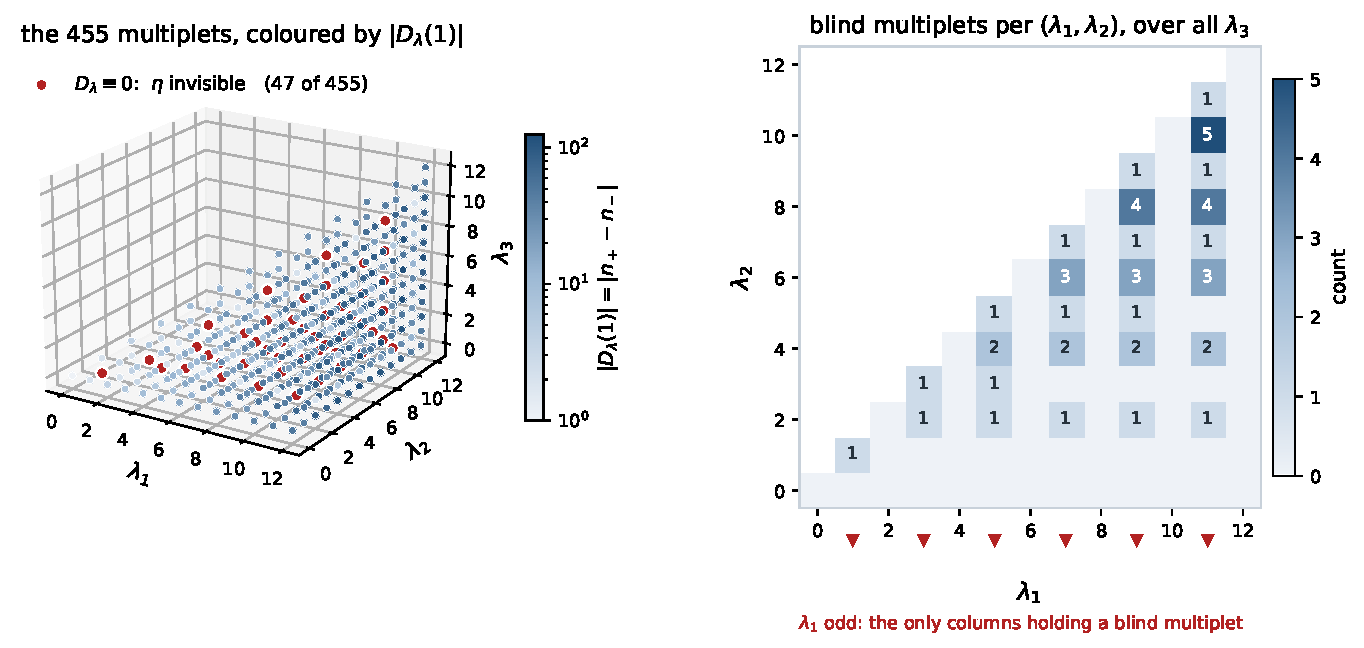
\includegraphics[width=\textwidth]{fig_blindclass.pdf}
\caption{The blind class, drawn from the archived sweep. \textbf{Left:} every $\su4$ multiplet with
$\lambda_1\le12$, $\lambda_4=0$, placed at $(\lambda_1,\lambda_2,\lambda_3)$ and coloured by the
magnitude $|D_\lambda(1)|=|n_+-n_-|$, the parity index of Part~IV, on a logarithmic ramp of one hue.
The $47$ multiplets of $\mathcal Z$ carry no magnitude at all and are drawn as their own class:
these are the ones whose boundary-condition sign $\eta$ no measurement of this Higgs sector can see.
\textbf{Right:} the same set projected on $(\lambda_1,\lambda_2)$, each cell counting the $\lambda_3$
that give a blind multiplet. The class is a structured surface, not scattered dust --- and the
structure is visible without any theory: \emph{no multiplet with $\lambda_1$ even is ever blind}
(\S\ref{sec:count}). Generated by \texttt{make\_figures.py} from
\texttt{outputs/fibre\_eta.json}; nothing is recomputed for the figure.}
\label{fig:blind}
\end{figure}

\subsection*{Why the two mechanisms are one}

Relation \eqref{eq:rel} degenerates --- sending $(\lambda,\eta)$ to $(\lambda,-\eta)$ --- exactly when
$\lambda$ is self-conjugate with $\lambda_1$ odd. With $\lambda_4=0$, self-conjugate means
$\lambda_2+\lambda_3=\lambda_1$, that is $\lambda_i+\lambda_{5-i}=\lambda_1$ for every $i$:
self-complementary of width $\lambda_1$. With $\lambda_1$ odd that is, word for word, branch~(b) of
Part~IV's vanishing criterion. So the degeneracy of the relation is not extra information; it is the
same statement seen twice [verified: $21$ of $21$ such irreducibles lie in $\mathcal Z$, out of $49$
self-conjugate ones in range].

\begin{figure}[t]
\centering
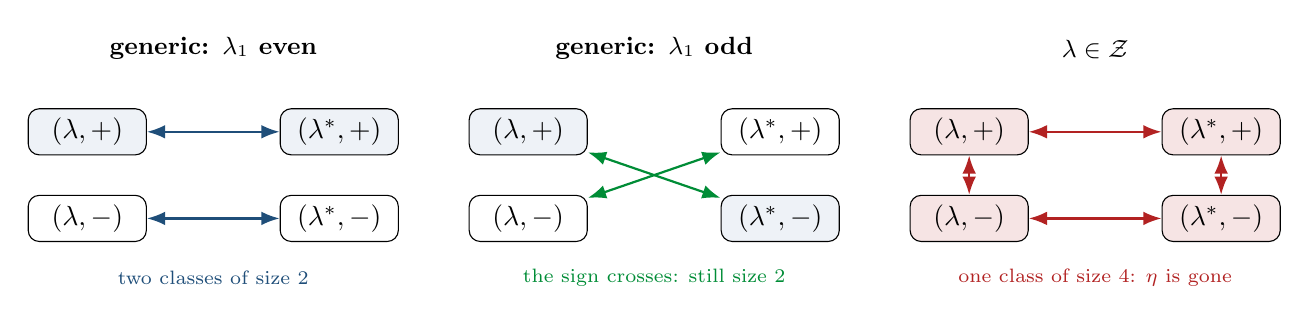
\begin{tikzpicture}[x=1cm,y=1cm,>=Latex]
\definecolor{cA}{RGB}{31,78,121}\definecolor{cB}{RGB}{0,140,54}\definecolor{cC}{RGB}{178,34,34}
% size 2 class
\begin{scope}[shift={(0,0)}]
\node[anchor=south] at (1.6,1.5) {\small\textbf{generic: $\lambda_1$ even}};
\node[draw,rounded corners,fill=softgrey,minimum width=1.5cm] (a1) at (0,0.7) {$(\lambda,+)$};
\node[draw,rounded corners,fill=softgrey,minimum width=1.5cm] (a2) at (3.2,0.7) {$(\lambda^*,+)$};
\node[draw,rounded corners,minimum width=1.5cm] (a3) at (0,-0.4) {$(\lambda,-)$};
\node[draw,rounded corners,minimum width=1.5cm] (a4) at (3.2,-0.4) {$(\lambda^*,-)$};
\draw[<->,cA,thick] (a1)--(a2); \draw[<->,cA,thick] (a3)--(a4);
\node[cA] at (1.6,-1.15) {\scriptsize two classes of size $2$};
\end{scope}
% size 2 class, lambda1 odd
\begin{scope}[shift={(5.6,0)}]
\node[anchor=south] at (1.6,1.5) {\small\textbf{generic: $\lambda_1$ odd}};
\node[draw,rounded corners,fill=softgrey,minimum width=1.5cm] (b1) at (0,0.7) {$(\lambda,+)$};
\node[draw,rounded corners,minimum width=1.5cm] (b2) at (3.2,0.7) {$(\lambda^*,+)$};
\node[draw,rounded corners,minimum width=1.5cm] (b3) at (0,-0.4) {$(\lambda,-)$};
\node[draw,rounded corners,fill=softgrey,minimum width=1.5cm] (b4) at (3.2,-0.4) {$(\lambda^*,-)$};
\draw[<->,cB,thick] (b1)--(b4); \draw[<->,cB,thick] (b3)--(b2);
\node[cB] at (1.6,-1.15) {\scriptsize the sign crosses: still size $2$};
\end{scope}
% Z
\begin{scope}[shift={(11.2,0)}]
\node[anchor=south] at (1.6,1.5) {\small\textbf{$\lambda\in\mathcal Z$}};
\node[draw,rounded corners,fill=cC!12,minimum width=1.5cm] (c1) at (0,0.7) {$(\lambda,+)$};
\node[draw,rounded corners,fill=cC!12,minimum width=1.5cm] (c2) at (3.2,0.7) {$(\lambda^*,+)$};
\node[draw,rounded corners,fill=cC!12,minimum width=1.5cm] (c3) at (0,-0.4) {$(\lambda,-)$};
\node[draw,rounded corners,fill=cC!12,minimum width=1.5cm] (c4) at (3.2,-0.4) {$(\lambda^*,-)$};
\draw[<->,cC,thick] (c1)--(c2);\draw[<->,cC,thick] (c3)--(c4);
\draw[<->,cC,thick] (c1)--(c3);\draw[<->,cC,thick] (c2)--(c4);
\node[cC] at (1.6,-1.15) {\scriptsize one class of size $4$: $\eta$ is gone};
\end{scope}
\end{tikzpicture}
\caption{The fibre of $(\lambda,\eta)\mapsto(\Sig,\eta\Dl)$, which is the observational equivalence
class. Shaded boxes lie in one class. The sign $\eta$ survives as an observable in the first two
panels and disappears in the third, and the third is exactly $\mathcal Z$: $D_\lambda\equiv0$ makes
$\eta$ act trivially there, on all $47$ multiplets of the class. A second route reaches the same
place --- when $\lambda$ is self-complementary of odd width, \eqref{eq:rel} degenerates and
identifies $(\lambda,+)$ with $(\lambda,-)$ by itself --- and it is not independent: those are
$21$ multiplets and all $21$ lie inside the $47$. No multiplet is blind to $\eta$ by any other
mechanism. Counts over $\lambda_1\le12$: $56+401+13$ classes of size $1,2,4$ covering all $910$
pairs.}
\label{fig:fibre}
\end{figure}

\subsection*{How big is the blind class}\label{sec:count}

Because Part~IV classifies $\mathcal Z$ in closed form, the blind set can be counted rather than
estimated, and the count has more structure than we expected. For fixed $\lambda_1$ the sweep is
complete --- $\lambda_2$ and $\lambda_3$ range over everything allowed --- so these are exact counts
and not samples:

\begin{center}\small
\rowcolors{2}{softgrey}{white}
\begin{tabular}{lccccccc}
\toprule
\rowcolor{hdrblue!12}
$\lambda_1$ & $1$ & $3$ & $5$ & $7$ & $9$ & $11$ & any even $\lambda_1$\\
\midrule
blind multiplets & $1$ & $2$ & $5$ & $8$ & $13$ & $18$ & \textcolor{warmred}{$0$}\\
$\lceil (k+1)^2/2\rceil$, $\lambda_1=2k{+}1$ & $1$ & $2$ & $5$ & $8$ & $13$ & $18$ & ---\\
\bottomrule
\end{tabular}
\end{center}

\noindent Both statements are consequences of Part~IV's criterion, and reading them off it is a
short argument rather than a debt:

\begin{proposition}\label{prop:count}
Let $\lambda=(\lambda_1,\lambda_2,\lambda_3,0)$. Then $\lambda\in\mathcal Z$ if and only if
\begin{enumerate}\itemsep1pt
\item[(a)] $\lambda_1$ odd, $\lambda_2$ even, $\lambda_3$ odd; \quad or
\item[(b)] $\lambda_1$ odd, $\lambda_2$ odd, $\lambda_3$ even and $\lambda_2+\lambda_3=\lambda_1$.
\end{enumerate}
The two cases are disjoint. In particular $\lambda_1$ is \emph{odd} for every $\lambda\in\mathcal Z$,
and for $\lambda_1=2k+1$
\[
\#\{\lambda\in\mathcal Z\}\;=\;\underbrace{\tfrac{k(k+1)}{2}}_{\text{(a)}}
\;+\;\underbrace{\lfloor k/2\rfloor+1}_{\text{(b)}}\;=\;\Big\lceil \tfrac{(k+1)^2}{2}\Big\rceil .
\]
\end{proposition}

\begin{proof}
The beta-set is $\beta=(\lambda_1+3,\lambda_2+2,\lambda_3+1,0)$, and Part~IV gives $D_\lambda\equiv0$
in exactly two situations: one parity class of $\beta$ is empty, or the split is $2+2$ and
$d_3=|a_1+a_2-b_1-b_2|=0$, where $\chi_{-1}=0$.

Since $\beta_4=0$ is even, the even class is never empty, so the first situation is that the odd
class is empty: $\lambda_1+3,\lambda_2+2,\lambda_3+1$ all even, which is (a).

For the second, the even class is $\{0,x\}$ with $x$ the unique even entry among
$\beta_1,\beta_2,\beta_3$. If $x=\beta_1$ then $\lambda_1$ is odd, the odd class is
$\{\lambda_2+2,\lambda_3+1\}$, and $d_3=0$ reads $\lambda_1+3=\lambda_2+\lambda_3+3$, which is (b).
If $x=\beta_2$ then $d_3=0$ reads $\lambda_2=\lambda_1+\lambda_3+2>\lambda_1$, contradicting
$\lambda_2\le\lambda_1$; if $x=\beta_3$ it reads $\lambda_3=\lambda_1+\lambda_2+4>\lambda_3$,
impossible. The cases are disjoint because $\lambda_2$ is even in (a) and odd in (b).

Counting at $\lambda_1=2k+1$. In (a), $\lambda_2=2j$ with $0\le j\le k$, and $\lambda_3$ odd with
$\lambda_3\le 2j$ leaves $\lambda_3\in\{1,3,\dots,2j-1\}$, that is $j$ values; summing gives
$k(k+1)/2$. In (b), $\lambda_3=\lambda_1-\lambda_2$ is determined and automatically even, and
$\lambda_2\ge\lambda_3$ is $2\lambda_2\ge 2k+1$, i.e.\ $\lambda_2\ge k+1$; the odd integers in
$[k+1,2k+1]$ number $(k+1)-\lceil k/2\rceil=\lfloor k/2\rfloor+1$. Finally
$k(k+1)/2+\lfloor k/2\rfloor+1=\lceil (k+1)^2/2\rceil$, by writing $k=2m$ and $k=2m+1$ separately.
\end{proof}

\noindent Figure~\ref{fig:blind} draws the class the proposition counts, and its right-hand panel is
the parity statement made visible: the populated columns are exactly the odd ones.

\noindent [Verified independently of the proof, on all $2925$ multiplets with $\lambda_1\le24$: the
characterisation disagrees with the exact computation of $D_\lambda$ in $0$ cases, the two branches
are disjoint, and each branch total is predicted separately --- branch~(a) $286$ against $286$
measured, branch~(b) $42$ against $42$.]

\subsection{The proposition is machine-checked, and it descends from Part~III's certificate}
\label{sec:lean}

Proposition~\ref{prop:count} is certified in Lean~4~\cite{Lean4} (\texttt{GHUBlindCount.lean},
Table~\ref{tab:leanV}). The point is not
that a counting argument has been re-typed in a proof assistant; it is \emph{where the certificate
starts}. Part~III already carries a machine-checked brick, \texttt{NotchCentreCharge.lean}, whose
main theorem is the vanishing criterion in Dynkin labels,
\[
N\,a\,b\,c=0\;\Longleftrightarrow\;\mathrm{Odd}\,b\wedge\big((\mathrm{Odd}\,a\wedge\mathrm{Odd}\,c)\vee a=c\big),
\]
proved by an honest Laplace expansion over $\mathbb{Z}[T;T^{-1}]$ with no \texttt{decide} on the
determinant. Part~V's proposition is stated in partition coordinates, and the passage between the
two is the substitution $a=\lambda_1-\lambda_2$, $b=\lambda_2-\lambda_3$, $c=\lambda_3$. That
substitution is exactly the step at which a paper of this kind silently goes wrong, so it is the
step we certified first: \texttt{blind\_iff\_N\_zero} closes the loop, and the count is therefore a
theorem \emph{about the determinant}, not about a predicate we invented to be countable.

It also settles, as a by-product, something the series had never checked mechanically. The proof of
Proposition~\ref{prop:count} above reads the two branches off \emph{Part~IV's} criterion --- the
parity classes of the beta-set and the $2{+}2$ split with $d_3=0$ --- while \texttt{blind\_iff\_notch}
proves those same two branches equivalent to \emph{Part~III's} criterion in Dynkin labels. The two
papers therefore describe one set, and the identification is now machine-checked rather than
assumed. It had been assumed since Part~IV.

Before a line of Lean was written the dictionary was swept in Python over the $39711$ partitions
with $\lambda_1\le 60$, with $0$ disagreements --- and, because a control that cannot fail is not a
control, the same sweep was run against a deliberately corrupted dictionary ($c:=b$), which it
rejects on $5200$ partitions.

\begin{table}[t]
\centering\small
\begin{tabular}{p{5.6cm}p{8.5cm}}
\toprule
\rowcolor{hdrblue}
\textcolor{white}{Lean theorem}\newline\textcolor{white}{(\texttt{GHUBlindCount.lean})} &
\textcolor{white}{content}\\
\midrule
\texttt{blind\_iff\_notch} &
the dictionary: on $\lambda_1\ge\lambda_2\ge\lambda_3$, branches (a)/(b) are the Dynkin criterion\\
\midrule
\rowcolor{softgrey}
\texttt{blind\_iff\_N\_zero} &
$\lambda\in\mathcal Z\leftrightarrow N(\lambda_1{-}\lambda_2,\lambda_2{-}\lambda_3,\lambda_3)=0$
--- the bridge to \texttt{NotchCentreCharge.lean}\\
\midrule
\texttt{blind\_l1\_odd} &
$\lambda\in\mathcal Z\Rightarrow\lambda_1$ odd; no even-$\lambda_1$ multiplet is ever blind\\
\midrule
\rowcolor{softgrey}
\texttt{card\_shellA}, \texttt{card\_shellB} &
branch~(a) $=$ the strict pairs $q<p\le k$, branch~(b) $=$ the interval $m\le\lfloor k/2\rfloor$;
(a) is stated doubled, $2\,\#(\mathrm a)=(k{+}1)k$, so no division on $\mathbb N$ enters the proof\\
\midrule
\texttt{card\_shell} &
$\#\{\lambda\in\mathcal Z:\lambda_1=2k{+}1\}=\lceil(k+1)^2/2\rceil$ --- Proposition~\ref{prop:count}\\
\bottomrule
\end{tabular}
\caption{The machine-checked core of Part~V, matter side. All statements are \texttt{sorry}-free and
depend only on \texttt{propext}, \texttt{Classical.choice}, \texttt{Quot.sound}. The parity of
$\lambda_2$ is what splits the shell into the two branches, so the case division of the paper proof
and the case division of the Lean proof are the same one. The geometry side --- the census of
\S\ref{sec:hhk}, Proposition~\ref{prop:census} --- is a second file,
\texttt{GHUCosetCensus.lean}, with the same standing and the same three axioms.}
\label{tab:leanV}
\end{table}

\paragraph{Where the certificate stops, exactly.} The chain is machine-checked from the bialternant
determinant onward. It is \emph{not} machine-checked back to the character: the identification
$D_\lambda(t)=s_\lambda(1,-1,t,t^{-1})=N/V$ is the classical bialternant definition of a Schur
function, used here as a classical input, together with $V\ne0$ (which \emph{is} certified, as
\texttt{V\_ne\_zero}). That boundary is not a matter of effort: Mathlib~\cite{Mathlib} has no Schur
functions at all --- it carries \texttt{YoungDiagram} and \texttt{SemistandardTableau}, and its three
files named for Schur are Schur's lemma, Schur--Zassenhaus and the Schur complement. Formalising
$s_{\lambda^*}(A)=\det(A)^{\lambda_1}s_\lambda(A)$, the complementation identity on which
Theorem~\ref{thm:main} rests, would require building that theory first, and we do not claim it.
Theorem~\ref{thm:main} is therefore proved but not certified; Proposition~\ref{prop:count} is both.

\subsection*{One step past a single multiplet, and it is free}

The certificate stops there; the \emph{statement} does not stop at a single multiplet, and the step
past it costs one line. A physical content is a multiset $\{(\lambda_i,\eta_i,n_i)\}$
with multiplicities $n_i>0$ and the observable is the sum, so two contents could still collide by a
cancellation that no pair of multiplets performs. Half of that possibility closes in one line. Write
$\zeta_i$ for the sign of Part~IV's closed form at $\lambda_i$, and call $\eta_i\zeta_i$ the
\emph{effective sign} of that multiplet.

\begin{proposition}[coherent signs]\label{prop:frust}
If every non-blind multiplet of a content carries the same effective sign, then
$\sum_i n_i\,\eta_i D_{\lambda_i}\equiv0$ if and only if every $\lambda_i$ is blind on its own.
\end{proposition}

\begin{proof}
Part~IV's closed form gives $D_{\lambda_i}=\zeta_i P_i$ with $P_i$ of non-negative coefficients, so
$\eta_iD_{\lambda_i}=(\eta_i\zeta_i)P_i$. If the effective signs share one value $\varepsilon$ the
sum is $\varepsilon\sum_i n_iP_i$, a sum of terms of one sign with positive weights, and it vanishes
only if every $P_i$ does.
\end{proof}

\noindent So \textbf{collective blindness requires sign frustration}: a content that is not blind
term by term can only go blind if it carries \emph{both} values of $\eta_i\zeta_i$. This does not
classify the frustrated case --- that is an integer kernel problem and it is the next paper --- it
removes the half that is structurally simple, and it carries the standing of Part~IV's identity, on
which the one-sign property rests.

\subsection*{What this section claimed in an earlier draft, and why it was wrong}

The first version of this section said: \emph{the coset half is the only observable in this model
that can see charge conjugation}. That is false, and it is contradicted in print. Kawamura, Kodaira,
Kojima and Yamashita~\cite{KKKY} write of the conjugate representation, in their \S5.1, ``which is
equivalent with the one of $\mathbf 4$. This holds for any representation'' --- and in their
formalism it is one line, since their potential is a sum of cosines and conjugation negates the
charges. Charge conjugation is invisible here \emph{unconditionally}.

The sign $(-1)^{\lambda_1}$ in \eqref{eq:rel} is real; what it speaks about is $\eta$. Because $U_6$
has $\det=-1$ it does not lie in $\su4$, so ``the character of $\bar R$ at $U_6$'' is not defined by
$\su4$ alone: it depends on which extension of the multiplet to the group generated by $\su4$ and
the determinant-flipping element is chosen, and the two natural extensions differ by exactly
$\det^{\lambda_1}$. That choice is the boundary condition. The statement that survives is
Theorem~\ref{thm:main}, and it is sharper than the one that died.

\bridge{The theorem is phrased in our own machinery, which is exactly the condition under which a
claim has not been gated at all. Said in the language the field has used since 2004, does it survive
--- and does it stay a statement about one six-dimensional model?}

% ===================================================================
\section{The same statement in the field's own variables}\label{sec:hhk}

Theorem~\ref{thm:main} is phrased in our machinery. It need not be, and the translation does more
than rename things: it shows the statement is a property of the five-dimensional classification of
boundary conditions and not of the particular model of \S\ref{sec:anchor}.

Haba, Hosotani and Kawamura~\cite{HHK} classify the boundary conditions of $\su N$ gauge theory on
$S^1/\ZZ_2$ by the block sizes $[p;q,r;s]$ of the two commuting parity matrices $P_0,P_1$, prove that
every equivalence class has a diagonal representative, and count the classes: $(N+1)^2$. For the
fundamental, the second-rank antisymmetric and the adjoint they tabulate (their eq.~(3.20)) the
multiplicities $N^{(\varepsilon_0,\varepsilon_1)}_{\mathrm{rep}}$ of basis vectors by their
$(P_0,P_1)$ parity. Those tables are three characters in disguise:

\begin{proposition}\label{prop:three}
For any representation of $\su N$ and any commuting pair of parities $(P_0,P_1)$,
\begin{keyeq}
\begin{equation}\label{eq:threechar}
N^{(\varepsilon_0,\varepsilon_1)}
=\tfrac14\Big[\dim+\varepsilon_0\,\chi(P_0)+\varepsilon_1\,\chi(P_1)
+\varepsilon_0\varepsilon_1\,\chi(P_0P_1)\Big].
\end{equation}
\end{keyeq}
\end{proposition}

\noindent Figure~\ref{fig:simplex} draws these three characters over the whole space of boundary
conditions, and shows that each layers it in a different direction.
Equation~\eqref{eq:threechar} is the trace of the projector
$\frac14(1+\varepsilon_0P_0)(1+\varepsilon_1P_1)$, and
it is verified against their printed table on every $[p;q,r;s]$ up to $N=8$: $1470$ cases, $0$
disagreements with eq.~(3.20) and $0$ with \eqref{eq:threechar}
[\texttt{hhk\_bridge.py}, output in \texttt{outputs/hhk\_bridge.txt}]. It is elementary, and it is
recorded here as a bridge and not as a discovery: what it buys is that the three numbers on the
right are the \emph{only} way a boundary condition enters, for every representation and not only for
the three that are tabulated.

Those three numbers are not new either, and the reader should meet their owners here. Takeuchi and
Inagaki~\cite{TI1,TI2} observed that a boundary-condition-connecting gauge transformation acts on the
rotation matrix at a fixed point by conjugation with $\Omega$ \emph{evaluated at that fixed point} ---
a constant --- so that the trace there is invariant by cyclicity, and they call the resulting
identities \emph{trace conservation laws}. With them they classify the equivalence classes on
$S^1/\ZZ_2$, $T^2/\ZZ_3$ and $T^2/\ZZ_m$ ($m=2,3,4,6$) without ever writing a gauge transformation,
recovering the counts and exhibiting off-diagonal classes. Their argument is representation-blind, so
$\chi_R$ at each fixed-point rotation matrix is a class invariant for \emph{every} $R$; we claim none
of that. Proposition~\ref{prop:three} is the projector count, a different use of the same three
numbers, and the two meet in \S\ref{sec:interp}.

\begin{figure}[t]
\centering
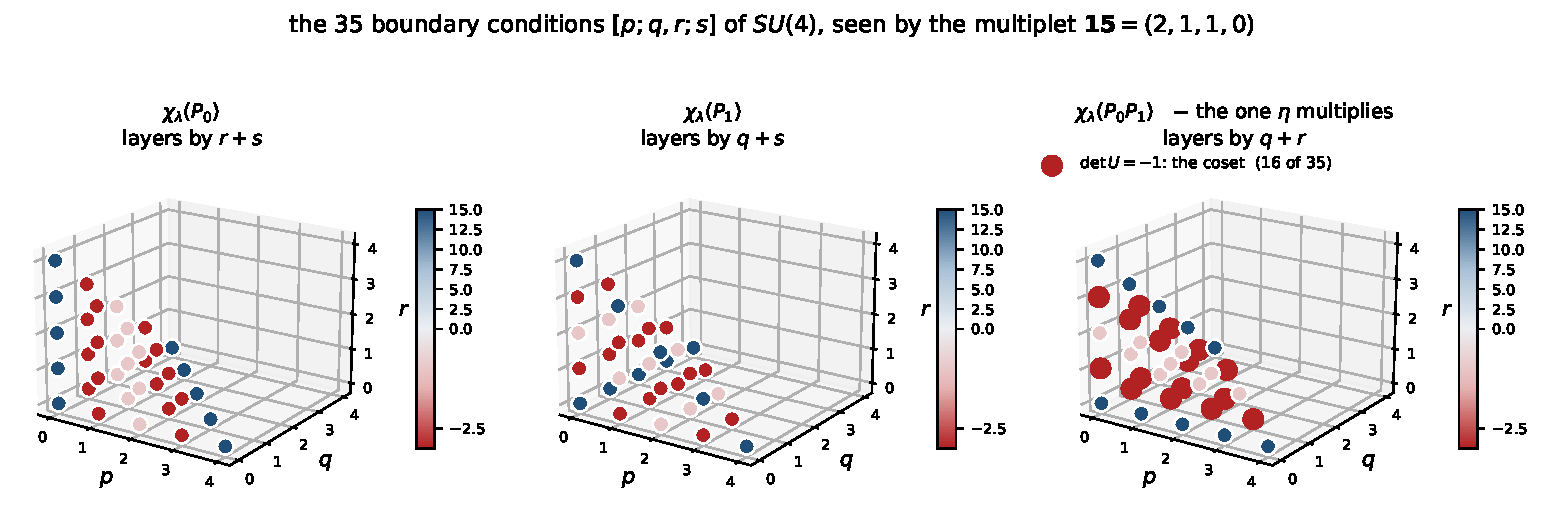
\includegraphics[width=\textwidth]{fig_simplex.pdf}
\caption{Proposition~\ref{prop:three} drawn. A boundary condition of $\su4$ on $S^1/\ZZ_2$ is four
non-negative integers $[p;q,r;s]$ summing to $4$, so the set of them \emph{is} a simplex with $35$
points; each is placed at $(p,q,r)$, with $s$ implied. The three panels colour the same simplex by
the three characters of \eqref{eq:threechar}, evaluated on the gauge adjoint. The colour job is
polarity, so the ramp is diverging with a neutral midpoint. \textbf{Each character layers the simplex
in a different direction} --- $\chi(P_0)$ depends on the block sizes only through $r+s$, $\chi(P_1)$
through $q+s$, and $\chi(P_0P_1)$ through $q+r$; all three layerings are verified, not asserted, in
\texttt{make\_figure\_simplex.py}. The third panel is the one that matters here: it is the character
the boundary sign $\eta$ multiplies, and the ringed points are the $16$ boundary conditions with
$\det U=-1$, the reflection coset --- the only place in this picture where $\eta$ can act at all.}
\label{fig:simplex}
\end{figure}

Turning on the boundary signs sends $(P_0,P_1)\mapsto(\eta_0P_0,\eta_1P_1)$, hence
$\varepsilon_i\mapsto\eta_i\varepsilon_i$ in \eqref{eq:threechar}. Two consequences follow by
inspection, and both are verified by sweep ($N\le6$, all $[p;q,r;s]$, three representations, $615$
cases, $0$ violations each):
\begin{enumerate}\itemsep2pt
\item $(\eta_0,\eta_1)\to(-\eta_0,-\eta_1)$ permutes the four multiplicities by
$(\varepsilon_0,\varepsilon_1)\to(-\varepsilon_0,-\varepsilon_1)$. This is their own sentence below
eq.~(4.3), here as an identity: the overall flip is a redundancy.
\item The finite part of their potential uses only the pair sums $N^{(++)}+N^{(--)}$ and
$N^{(+-)}+N^{(-+)}$ (their $N_v$ in eq.~(3.25), and eqs.~(4.11)--(4.13)), and these are
$\frac12[\dim\pm\eta_0\eta_1\chi(P_0P_1)]$: they depend on the boundary signs \emph{only} through the
product $\eta=\eta_0\eta_1$, and they distinguish its two values exactly when $\chi(P_0P_1)\neq0$.
\end{enumerate}
The individual sign $\eta_0$ survives only in their $N_\xi$ term, and $\xi$ is the divergent quantity
they themselves declare incomparable between equivalence classes. Everything finite sees the
product. This is why \eqref{eq:etaname} is a definition and not an approximation.

So $\eta$ is invisible to a multiplet precisely when the character at the winding element
$U=P_0P_1$ vanishes. For $\su4$, $\det U=(-1)^{q+r}$, so $U$ lies in the reflection coset exactly
when $q+r$ is odd --- $16$ of the boundary conditions, and $U$ then has only two spectra,
$\mathrm{diag}(1,1,1,-1)$ and $\mathrm{diag}(-1,-1,-1,1)$, the conjugacy class of Part~III's parity
matrix $P_0$. Hence $\chi_\lambda(U)=s_\lambda(1,1,1,-1)=\Dl(1)$ and Theorem~\ref{thm:main} reads, in
their variables: \emph{$\eta_0\eta_1$ is invisible to $\lambda$ if and only if $\chi_\lambda(U)=0$.}

\subsection{The Wilson line interpolates the trace conservation laws}\label{sec:interp}

The two readings meet, and the meeting point is the sharpest sentence we can make about our own
object. A trace conservation law is a number: the character at a fixed-point rotation matrix. Our
$\Dl$ is a \emph{function} of the Wilson line phase, and at $t=1$ it is
$\chi_\lambda(\mathrm{diag}(1,1,1,-1))$ --- the character at Part~III's parity matrix, that is,
exactly a trace conservation law for the representation $\lambda$. So the two Schur specialisations
of \eqref{eq:SigD} interpolate the conserved traces: the invariants of~\cite{TI1,TI2} are the
endpoints, and the Wilson line phase is what runs between them. The theorem of \S\ref{sec:obs} then
says that the boundary sign is invisible exactly where that interpolating function is identically
zero --- and the corollary below says that this is already decided at the endpoint.

\subsection*{A difference of regime that turns out not to exist}

Their formulas are evaluated at vanishing Wilson line phase, where the sign multiplies the number
$\Dl(1)$; ours lives at a dynamical phase, where it multiplies the polynomial $\Dl(t)$. A priori
$\Dl(1)=0$ is the weaker condition and should define a strictly larger class of blind multiplets. It
does not.

\begin{corollary}\label{cor:regime}
$\Dl(1)=0\iff\Dl\equiv0$. The boundary-condition sign is invisible at vanishing Wilson line phase if
and only if it is invisible at every phase, and both conditions are $\mathcal Z$.
\end{corollary}

\begin{proof}
Part~IV's closed form gives $\delta(m)=\zeta\cdot(\text{non-negative})$ with a single global sign
$\zeta$, so all coefficients of $\Dl=\sum_m\delta(m)t^m$ carry the same sign; a sum of terms of one
sign vanishes only if every term vanishes.
\end{proof}

\noindent In the language of \S\ref{sec:interp}: \emph{a single conserved trace controls the whole
interpolating function}, and it does so because Part~IV's closed form gives the coefficients one
sign --- so this corollary carries that identity's standing, and no more.

\noindent [Verified over the $455$ irreducibles in range: $0$ have coefficients of both signs;
$\Dl(1)=0$ on $47$ and $\Dl\equiv0$ on the same $47$, with $0$ in either class and not the other.]

The practical consequence is that the theorem can be quoted to a five-dimensional reader and a
six-dimensional one without changing a word.

\subsection*{What is theirs}

Stated plainly, because the neighbourhood is theirs: the classification $[p;q,r;s]$, the equivalence
relation $[p;q,r;s]\sim[p-1;q+1,r+1;s-1]$, the count $(N+1)^2$, the diagonal-representative theorem,
the generic one-loop potential at vanishing Wilson line phase, and the redundancy
$(\eta_0,\eta_1)\sim(-\eta_0,-\eta_1)$ are all in~\cite{HHK}. So is a blindness of the potential:
they observe that their eq.~(4.13) ``is a function of $q+r$ only'' and ``does not select unique
$[p;q,r;s]$'', and close the paper saying the arbitrariness problem is unsolved because ``there
remains a degeneracy among the theories of the lowest energy density''. That degeneracy is on the
side of the boundary-condition \emph{labels}. Ours is on the side of the matter \emph{content} ---
which multiplets cannot see $\eta$ --- and the two are complementary, in the same spirit, and not the
same statement. What is added here is Proposition~\ref{prop:three} for general representations,
where they tabulate three by hand, and the closed-form identification of the blind class.

\subsection*{When a model has an index sector at all, and how often}

The root of \S\ref{sec:spine} is a test, and it is a test on the \emph{embedding} rather than on the
matter: a coset sector exists if and only if $\det P_0\neq\det P_1$. In the $[p;q,r;s]$ labels that is
$\det U=(-1)^{q+r}$, and the parity of $q+r$ is a class invariant --- the equivalence move sends
$q+r\mapsto q+r+2$. So the question can be counted, not just posed:

\begin{center}\small
\rowcolors{2}{softgrey}{white}
\begin{tabular}{rrrr}
\toprule
\rowcolor{hdrblue!14}$N$ & classes $(N+1)^2$ & with an index sector & without\\
\midrule
$2$ & $9$ & $4$ & $5$\\
$3$ & $16$ & $8$ & $8$\\
$4$ & $25$ & $12$ & $13$\\
$5$ & $36$ & $18$ & $18$\\
$\vdots$ & & & \\
$10$ & $121$ & $60$ & $61$\\
\bottomrule
\end{tabular}
\end{center}

\noindent The pattern is exact, and it is a theorem rather than a sweep. The move leaves
$(p+q,\,q+s)$ --- that is, $(\#\{P_0=+1\},\,\#\{P_1=-1\})$ --- untouched, and that pair is a
\emph{complete} invariant: two block patterns with the same $N$ and the same pair are joined by a
chain of moves, because the pair itself leaves room for each step. So the classes of rank $N$ are
exactly the pairs $(u,v)$ with $u,v\le N$, which is \cite{HHK}'s $(N+1)^2$ recovered, and
$q+r\equiv u+v+N \pmod 2$, which is what makes ``has a coset sector'' a property of the class.

\begin{proposition}[the census]\label{prop:census}
Of the $(N+1)^2$ equivalence classes of boundary conditions of $SU(N)$ on $S^1/\ZZ_2$, exactly
$\lfloor (N+1)^2/2\rfloor$ admit a reflection-coset sector, and in the other
$\lceil (N+1)^2/2\rceil$ the boundary sign is invisible to \emph{every} multiplet.
\end{proposition}

\noindent Both halves are machine-checked in Lean~4~\cite{Lean4}
(\texttt{GHUCosetCensus.lean}, \texttt{sorry}-free, the same three axioms as
Table~\ref{tab:leanV}): \texttt{label\_move} and \texttt{eqv\_of\_label} for the complete invariant,
\texttt{coset\_parity} for the class function, and \texttt{card\_cosetClasses} for the count, for
every $N$ and not for the ten in the table. The controls are in the file and they can fail: the
equally natural label $(p+q,q+r)$ is \emph{not} move-invariant, the other parity class has the other
cardinal, and a brute-force enumeration of every $[p;q,r;s]$ of rank three returns exactly the grid
the theorem predicts.

\emph{This census is an $S^1/\ZZ_2$ statement and stays one.} It is legitimate there because every
equivalence class has a diagonal representative --- that is \cite{HHK}'s Appendix~A, and without it
the count would be over representatives rather than classes. The corresponding classification on the
two-dimensional orbifolds, including the $T^2/\ZZ_2$ of this model, is Kawamura and
Miura's~\cite{KM}, and there the diagonal assumption is \emph{not} free: they exhibit boundary
conditions that cannot be simultaneously diagonalised at all. We therefore do not carry the count
across, and \S\ref{sec:scope} says so.

This closes the invisibility question into two disjoint cases, and only the second is ours:

\begin{center}
\fcolorbox{hdrblue!55}{hdrblue!6}{\begin{minipage}{0.88\textwidth}
\emph{The boundary-condition sign $\eta$ is invisible either because the geometry has no coset sector
--- $\det P_0=\det P_1$, roughly half of all classes, and then it is invisible to \textbf{every}
multiplet --- or because the matter is parity-balanced, which is Theorem~\ref{thm:main} and Part~IV's
class $\mathcal Z$.}
\end{minipage}}
\end{center}

\noindent The first case is a one-line check a model builder can run before anything else; the second
needs the closed form. Stating both is what makes the answer complete rather than merely true.

\bridge{Every section so far has been about what a boundary condition \emph{is}. The variable that
decides which part of one is physical has been present in every formula and has never once been the
subject; \S\ref{sec:wilson} makes it one.}

% ===================================================================
\section{The Wilson line, and what it can and cannot absorb}\label{sec:wilson}

The Wilson line has appeared in every section as a variable and has not once been the subject. It is
the connective tissue of the whole construction, and the pieces above say five distinct things about
it.

\textbf{It is the Higgs.} Not an analogue: the physical degrees of freedom are the gauge-invariant
phases of $W=P\exp(ig\oint A_y\,dy)$. At tree level the potential is flat along them --- they
parametrise degenerate vacua --- and the degeneracy is lifted only at one loop. That is the Hosotani
mechanism~\cite{Hosotani}, and it is the entire electroweak sector of this model.

\textbf{It is the continuous half of the holonomy.} The winding amplitude is the character at
$\exp(i\pi\theta T)\,U_6^{\,k_2}$: a \emph{continuous} Wilson line times a \emph{discrete} orbifold
twist. The discrete factor takes only two values in $O(4)$, and that is the $\ZZ_2$ of
\S\ref{sec:onez2}; the continuous factor is $t$, and it is what makes each half a \emph{function}
rather than a number. Everything Part~IV established is a statement about that function, uniform in it.

\textbf{It absorbs exactly the part of a boundary condition that is not physical.} Two boundary
conditions in one equivalence class are related by a transformation that \emph{changes} them, and the
equivalence holds because the Wilson line shifts to compensate --- point~(v) of the Hosotani
mechanism as~\cite{HHK} state it. That is why the trace conservation laws of~\cite{TI1,TI2} are
conserved: at a fixed point the transformation is conjugation by a constant, which the Wilson line
cannot reach. Measured on the classification:

\begin{center}\small
\rowcolors{2}{softgrey}{white}
\begin{tabular}{lll}
\toprule
\rowcolor{hdrblue!14}datum & under the class move & absorbed by\\
\midrule
$\mathrm{Tr}\,P_0$, $\mathrm{Tr}\,P_1$ & invariant & nothing --- they \emph{are} the class\\
$q+r$ & $\mapsto q+r+2$ & the Wilson line\\
parity of $q+r$, i.e.\ $\det U$ & invariant & nothing --- it decides whether a coset sector exists\\
\bottomrule
\end{tabular}
\end{center}

\noindent [all three rows are proved for every $N$, by Proposition~\ref{prop:census}]. \emph{The class invariants are precisely what the Wilson
line cannot absorb.}

\textbf{It interpolates the conserved traces.} Theirs are numbers at fixed points; ours is a
function, and $\Dl(1)$ \emph{is} one of their invariants (\S\ref{sec:interp}). Corollary
\ref{cor:regime} then says something sharp about the interpolation: for this object the Wilson line
carries \emph{no} information about vanishing --- the endpoint already decides it --- while carrying
all of it about magnitude.

\textbf{And it is the obstruction between a closed-form potential and a closed-form Higgs mass.}
$V(\alpha)$ is closed-form for arbitrary content (\S\ref{sec:two}); the only transcendental step left
is minimising over $\alpha$. That is where this paper stops, and the reason is worth recording.

\emph{A draft of this section reported a measurement here --- that at the vacuum the coset half
carries the whole Higgs curvature --- and it did not survive its own instrument check: the assembly
which produced it missed AHMN's published mass matrix, and on the corrected one the pattern is gone.
The full record, and the corrected instrument, open Part~VI. What survives of this section is its
structure, not that measurement.}

\noindent What survives is the negative that motivated the search and is unaffected by it: the Dynkin
index does not fix the Higgs curvature at the vacuum, because it is the $\alpha\to0$ limit and the
Wilson line has moved the system elsewhere. \emph{Which half carries the mass is open, and it is not
this paper's question} --- see \S\ref{sec:scope}.

\medskip
One distinction not to blur, since the two are easy to conflate and the literature warns against it:
$\alpha$ is continuous, gauge-invariant and \emph{is} the Higgs; $\eta$ is a discrete boundary phase.
They enter differently --- $\alpha$ as the argument of both halves, $\eta$ as a multiplier on the
coset half alone --- and that difference is the reason \S\ref{sec:obs} has anything to say.

\bridge{That is the structure, end to end. What it is \emph{for} --- and what it says to a problem
the field has had open for twenty-two years --- is the next section, and the last one that claims
anything.}

% ===================================================================
\section{The reading}\label{sec:reading}

The declared open problem of this field --- four groups over twenty-two years --- is that no known
mechanism selects among equivalence classes of boundary conditions. Hosotani named it the
arbitrariness problem~\cite{HosotaniArb}; \cite{HHK} attacked it by comparing vacuum energy densities and reported that
a degeneracy survives; \cite{KKKY} is still working the same seam.

Theorem~\ref{thm:main} speaks to it from the other side. It does not select a boundary condition. It
says exactly \emph{which multiplets cannot help you select one}, because for them the choice is
invisible in principle --- and it identifies that set with a criterion Part~IV already classified in
closed form, with no hypothesis on the shape of the partition, and which
Proposition~\ref{prop:count} counts. A model builder choosing bulk matter
to make a boundary condition dynamically preferred now has a test that costs nothing: if the content
lies in $\mathcal Z$, the coset half is empty and the content is inert with respect to $\eta$, no
matter how the rest of the model is arranged.

\subsection*{What changes for someone building one of these models}

The rest of this section is the practical content, stated as four consequences with the limit of
each attached, because an implications section is where a paper overclaims if it is allowed to.

\textbf{1. A selection rule on bulk matter, applicable by inspection.} Given a Young diagram,
Proposition~\ref{prop:count} decides in closed form whether that multiplet lies in $\mathcal Z$. If
it does, the multiplet contributes \emph{nothing} to the coset half: it cannot help select a boundary
condition, and it enters the breaking criterion \eqref{eq:crit} through its Dynkin index alone. That
is a constraint one can apply before computing anything. \emph{Limit:} it is per multiplet --- a
content is a multiset, and cancellations between multiplets are covered only where the effective
signs agree (Proposition~\ref{prop:frust}); the frustrated case is not.

\textbf{2. The potential of an arbitrary multiplet, without a Kaluza--Klein spectrum.} The
published treatments obtain the mode list per representation --- \cite{HY} for the adjoint,
fundamental and (anti)symmetric tensors, \cite{AHMN} and \cite{KKKY} by hand from the spectrum. Here
it is read off $\lambda$ for \emph{any} irreducible, through the same universal $G$
(\S\ref{sec:two}). The practical consequence is arithmetic: a scan over matter content stops being
limited to the handful of representations whose spectra somebody has written out. \emph{Limit:} a
closed form for the potential is not a closed form for the Higgs mass, which needs the minimum.

\textbf{3. A one-line test on the embedding, before any matter is chosen.} A coset sector exists at
all only when $\det P_0\neq\det P_1$, and $\lfloor(N+1)^2/2\rfloor$ of the $(N+1)^2$ equivalence
classes are of that kind (\S\ref{sec:hhk}). In the other half the boundary-condition sign is
invisible to \emph{every} multiplet, for reasons that have nothing to do with the matter. The count
is Proposition~\ref{prop:census} and holds for every $N$. \emph{Limit:} it is an $S^1/\ZZ_2$ count,
and diagonal boundary conditions only.

\textbf{4. The two halves answer different questions, and that splits the next problem cleanly.} The
even-winding half determines the matter up to conjugation; the odd-winding half carries the boundary
sign. For a content rather than a multiplet this matters, because the coefficients of $\Sig$ are
non-negative (\S\ref{sec:two}) and therefore a sum of them \emph{cannot cancel}: two contents with
the same even half are two decompositions of one non-negative function, an additive question with no
cancellation in it. The odd half is where genuine cancellation between multiplets lives --- and by
Proposition~\ref{prop:frust} it needs \emph{sign frustration} to live there at all: with one
effective sign $\eta_i\zeta_i$ throughout, the odd half cannot cancel either, and the content is
blind only if every multiplet in it is. Whoever attacks the degeneracy of contents should attack
those two halves separately, and inside the odd one, only the frustrated case; they are not the same
problem. \emph{Limit:} the separation statement for $\Sig$ is verified on $969$ multiplets and not
proved (\S\ref{sec:scope}).

\textbf{5. The weight in the breaking criterion is geometry, not a parameter.} $\rho=7.5115$ is
fixed by the fall-off of the winding sum, hence by the dimension of the compactification, because the
shortest winding that contributes to the curvature is odd (\S\ref{sec:halves}). It is not available
for tuning --- and it also says how fragile a verdict is: the base $\mathbf{60}$ of this model sits at
a critical $\rho=6.4545$ against an actual $7.5115$, so a $14.1\%$ shift reverses it. Verdicts within
that margin should be quoted with it.

\medskip
Part~III exported a question about symmetric functions. The answer comes back as a statement about
which part of the matter content is observable in principle: \emph{the vanishing class is where the
boundary condition stops mattering.}

\bridge{Everything claimed here is negative --- what cannot be seen, and therefore cannot be wrong.
Running the same machinery \emph{forwards}, to predict a Higgs spectrum rather than to rule one out,
is a different kind of claim and a more fragile one. It is the subject of the sequel and is
deliberately not in this paper. What is owed here are the limits.}

% ===================================================================
\section{Scope, and what is open}\label{sec:scope}

\textbf{Proved.} Relation \eqref{eq:rel}, on any inversion-stable alphabet and for any number of
reciprocal pairs. The identification of its degenerate case with branch~(b) of Part~IV.
Proposition~\ref{prop:three}. Proposition~\ref{prop:count}, machine-checked, and with it the
vanishing criterion itself --- Part~III's theorem in Dynkin labels, whose dictionary with the
partition form \S\ref{sec:lean} certifies. Proposition~\ref{prop:census}, machine-checked, and with
it the completeness of $(\#\{P_0{=}+1\},\#\{P_1{=}-1\})$ as a class invariant: the census holds for
every $N$, where the paper's table only sweeps ten.

\textbf{Proved on an identity that is itself verified and not proved.} Corollary~\ref{cor:regime},
and every one-sign argument, needs Part~IV's closed form to give $\Dl$ coefficients of a single sign,
and Part~IV states that identity as an Observation. What does \emph{not} depend on it is the
criterion the identity computes, so $\mathcal Z$, its count and its Lean certificate stand
regardless; only the sentence that $\mathcal Z$ is the \emph{zero locus} of $\Dl$ would have to be
re-read.

\textbf{Verified, not proved --- and now reduced to one function and one residual case.}
Observation~\ref{obs:complete}: that \eqref{eq:rel} generates \emph{all} collisions is verified with
$0$ exceptions among $910$ pairs, and unproved. Three measurements sharpen the problem considerably, and they are worth stating because
they turn a search into a question.

First, the pair is not needed: \emph{$\Sig$ alone separates}. Over the $969$ multiplets with
$\lambda_1\le16$ its fibres have sizes $\{1:81,\,2:444\}$, the $81$ singletons are exactly the $81$
self-conjugate multiplets, and \emph{no} fibre fails to be the conjugation orbit $\{\lambda,\lambda^*\}$.
So the question is about one symmetric function, not two.

Second, two of the three parameters come out in closed form, and both are conjugation-invariant as
they must be: the top exponent of $\Sig$ is $\lambda_1$, and its top $SU(2)$ coefficient is
$\lambda_2-\lambda_3+1$ [both $0$ failures on all $455$ multiplets with $\lambda_1\le12$]. Since
$\lambda^*=(\lambda_1,\lambda_1-\lambda_3,\lambda_1-\lambda_2,0)$ leaves $\lambda_1$ and
$\lambda_2-\lambda_3$ fixed, neither could have distinguished the orbit, and neither does.

Third, what is left is $\lambda_2+\lambda_3$ modulo the reflection
$s\mapsto2\lambda_1-s$ that conjugation induces --- and the next two coefficients do \emph{not}
determine it. There are $28$ collisions, and they are all of one shape: the family
$\lambda=(\lambda_1,k,k,0)$ has the same first three $SU(2)$ coefficients for every $k$. The full
coefficient sequence does separate them; a proof has to reach past the top of the list, and the
residual case is now named.

\textbf{Per multiplet.} A physical content is a multiset of irreducibles with multiplicities and the
observable is the \emph{sum}, so distinct contents may still collide by cancellation even when no two
multiplets do --- but only with both effective signs present, by Proposition~\ref{prop:frust}. How
large that frustrated degeneracy is, and what generates it, is open and is the next paper.
The tools for it are exact ones --- integer linear programming over the anomaly and tadpole
constraints, quotiented by the invisible group identified here --- and the moment tower
$M_{2r}=\sum_m\delta(m)(m^2)^r$ is a signed sum of geometric sequences, so its Hankel matrix has rank
equal to the number of distinct winding charges and a generalised eigenvalue problem returns those
charges exactly, with integer eigenvalues [\texttt{hankel\_probe.py}].

\textbf{Not claimed.} That the potential distinguishes $R$ from $\bar R$: it does not, see
\S\ref{sec:obs}, and the literature says so first. That anything here is about nature: every
statement is about a model, on $T^2/\ZZ_2$ with $U_5=\one$, at one loop.

\textbf{Diagonal boundary conditions only, and we did not know this until we read for it.} Every
statement above assumes the orbifold parities can be simultaneously diagonalised, which on $S^1/\ZZ_2$
is no restriction --- Haba, Hosotani and Kawamura prove every equivalence class has a diagonal
representative~\cite{HHK}. On $T^2/\ZZ_2$, the geometry of this model, it \emph{is} a restriction:
Kawamura and Miura~\cite{KM} exhibit boundary conditions for $\su N$ ($N\ge3$) that cannot be brought
to diagonal form by any global unitary together with a local gauge transformation, and note that a
multiplet's components then fail to be simultaneous eigenstates of the $\ZZ_2$ parities. The two
alphabets of \eqref{eq:alphabets} presuppose a diagonal winding element. Nothing here applies to the
off-diagonal classes, and we make no claim about them.

\textbf{Deliberately not here: everything that runs the machinery forwards.} Which half carries the
Higgs mass at the vacuum, what a given matter content predicts for $\alpha_{\min}$ and $\kappa_V$,
and how large the degeneracy becomes once contents carry multiplicities --- all of that is an open
search, and a closed theorem and an open search do not belong in one paper. They are Part~VI. This
paper is the closed half, and every statement in it is either proved or exhaustively verified in a
stated range.

\textbf{And the standing lesson, since it has now cost us twice.} A measured pattern is worth
nothing until the instrument that measured it reproduces something published. Ours reproduced
AHMN's \emph{vacuum} approximately and their \emph{mass matrix} not at all, and the difference was a
twist recorded in our own archived output and never applied.

\textbf{A neighbouring literature, and what it does and does not say about this.} $C^\star$ boundary
conditions~\cite{Cstar} make fields periodic \emph{up to charge conjugation}, so that one trip round
the torus applies an automorphism that is not inner. Three features there have the shape of what is
above: a $\ZZ_2$ survives the twist (electric charge is not conserved, but $(-1)^Q$ is, their
eq.~(2.26)); the effect comes entirely from a particle that winds at least once; and the boundary
data is a set of discrete signs modulo one overall redundancy (their eq.~(6.7)). We take the framing
and claim nothing from it: their $\ZZ_2$ is a \emph{conservation law on states} --- charged states
cannot mix with the vacuum --- whereas the winding parity here is a \emph{grading of a sum}, an index
of summation rather than a quantum number. The shape is shared; the statement is not, and we do not
borrow it.

\textbf{Untouched.} The viability of the $(3,60)$ content under the boundary-mass filter, which is a
question of Part~I and is not addressed by anything above. And the cosmological-constant question is
not ours to touch: the winding sum excludes $k=0$, and the $k=0$ term is exactly the
$\alpha$-independent piece that would be it.

% ===================================================================
\section{Ledger}\label{sec:ledger}

Item by item, as in Parts~III and IV. Non-negotiable, and rebuilt whenever the paper moves.

\begingroup\small
\renewcommand{\arraystretch}{0.90}  % the ledger pays for the scope paragraph, or the bibliography widows
\rowcolors{2}{softgrey}{white}
\setlength{\LTpre}{4pt}\setlength{\LTpost}{4pt}
\begin{longtable}{p{7.1cm} p{8.1cm}}
\toprule
\rowcolor{hdrblue!14}\textbf{Inherited} & \textbf{Source}\\
\midrule
\endfirsthead
\toprule
\rowcolor{hdrblue!14}\textbf{Ledger, continued} & \textbf{Source, evidence, or reason}\\
\midrule
\endhead
The Hosotani mechanism; Wilson-line phases as physical degrees of freedom & \cite{Hosotani}\\
The orbifold construction, chiral fermions and the split multiplet & \cite{Kawamura,HallNomura}, with
\cite{SS} for the supersymmetry-breaking twist\\
Boundary-condition equivalence classes on $S^1/\ZZ_2$; $[p;q,r;s]$; the count $(N+1)^2$; the
diagonal-representative theorem; the redundancy $(\eta_0,\eta_1)\sim(-\eta_0,-\eta_1)$; the
arbitrariness problem & \cite{HHK}, \cite{HosotaniArb}\\
The classification on the two-dimensional orbifolds, and the existence of boundary conditions that
cannot be simultaneously diagonalised & \cite{KM}\\
Trace conservation laws: the character at a fixed-point rotation matrix is an equivalence-class
invariant, and the classification built on them & \cite{TI1,TI2}\\
A general one-loop potential per representation class, and the method that extends it & \cite{HY};
the closest two-phase computation, \cite{HHHK}\\
The published one-loop potential of the 6D $\su4$ model and its coefficients $\{A+B(-1)^{k_2}\}$ &
\cite{AHMN}\\
That charge conjugation is invisible in this class of models & \cite{KKKY}\\
The centre-charge grading of the Wilson-line potential & \cite{DM}, \cite{RW},
\cite{ArgyresUnsal,Ogilvie}\\
That a root-of-unity specialisation makes a character vanish off the $t$-core and factor over the
$t$-quotient & Littlewood--Richardson, and \cite{Lecouvey,AK,Albion} --- none of them our alphabet\\
The twining reading of a character on a non-identity component & \cite{Jantzen,KLP}, via Part~IV\\
A non-inner boundary twist, and discrete boundary signs modulo one redundancy, as standard practice &
\cite{Cstar}\\
The closed form for $s_\lambda(1,-1,t,t^{-1})$, its vanishing criterion, and $\zeta$ as a parity
index & Part~IV \cite{PartIV}, which states the closed form as \emph{verified, not proved}\\
The mode labels, $U_6=P_2P_0^{-1}$, the notch and the decoupling corollary & Part~III \cite{PartIII}\\
\midrule
\rowcolor{okgreen!16}\textbf{Ours} & \textbf{Where, and on what evidence}\\
\midrule
Winding parity is the $O(4)$ component label, so the potential is $(\Sig,\Dl)$; and $\det P$ is
pinned by $P^2=\one$, not chosen & \S\ref{sec:spine}--\ref{sec:two}\\
Equation~\eqref{eq:tracepair}: the two halves are one operator traced twice, $\mathrm{Tr}(g)$ and
$\mathrm{Tr}(\sigma g)$ --- a dimension and an index & \S\ref{sec:two}, $287$ checks, $0$ failures\\
Both halves as stacks of one universal box; the identity half as a positive superposition, with a
summation range that is not a choice & \S\ref{sec:two}, $286/286$, $2197/2197$\\
Why one half factors and the other cannot: the frozen letters are roots of unity, so every zero of
$D$ lies on the unit circle and essentially none of $\Sigma$'s do --- and the \emph{control}, the
repeated-letter blocks, is ours & \S\ref{sec:two}, Figure~\ref{fig:zeros}\\
The dictionary $A=\tfrac12(\Sigma+D)$, $B=\tfrac12(\Sigma-D)$, and the published coefficients of
three separate papers reproduced from representation theory & \S\ref{sec:anchor}; \cite{AHMN} twelve
numbers, \cite{HY} four printed objects, \cite{HHHK} two of three representations\\
$\rho=7.5115$ is geometry and not a coupling: the shortest winding that contributes to the curvature
is odd & \S\ref{sec:halves}, control at $0.3443$\\
Theorem~\ref{thm:main}: the classes of $(\lambda,\eta)$, and $\eta$ blind exactly on $\mathcal Z$ &
\S\ref{sec:obs}, $910\to470$, $0$ unexplained\\
Proposition~\ref{prop:count}: $\mathcal Z$ characterised and counted, $\lceil(k+1)^2/2\rceil$ and
never $\lambda_1$ even & \S\ref{sec:lean}, \textbf{\color{okgreen}Lean 4}; $0$ disagreements on $2925$\\
Corollary~\ref{cor:balance}: $\mathcal Z$ is level-by-level parity balance & \S\ref{sec:two},
$47=47$\\
Proposition~\ref{prop:three}: a boundary condition sees a representation through three characters &
\S\ref{sec:hhk}, $1470$ cases, $0$ mismatches\\
Corollary~\ref{cor:regime}: the two regimes are one condition & \S\ref{sec:hhk}, $47=47$\\
Proposition~\ref{prop:frust}: collective blindness requires sign frustration & \S\ref{sec:obs}, one
line from Part~IV's one-sign property, and with its standing\\
Proposition~\ref{prop:census}, the census: $\lfloor(N+1)^2/2\rfloor$ of the $(N+1)^2$ classes admit a
coset sector, splitting invisibility into a geometric case and a matter case &
\S\ref{sec:hhk}, \textbf{\color{okgreen}Lean 4}; every $N$, not the ten in the table\\
That $\Sig$ alone separates the multiplet up to conjugation, with $\lambda_1$ and
$\lambda_2-\lambda_3$ recovered in closed form --- \emph{verified, not proved} & \S\ref{sec:scope},
$969$ multiplets, $0$ exceptions\\
\midrule
\rowcolor{warmred!14}\textbf{Retracted, and left visible} & \textbf{Why}\\
\midrule
``The coset half is the only observable that sees charge conjugation'' & false, and \cite{KKKY} say
so in print. \S\ref{sec:obs}\\
``At the vacuum the coset half carries the whole Higgs curvature'' & an artefact of an assembly that
missed \cite{AHMN}'s mass matrix. \S\ref{sec:scope}, and Part~VI\\
\bottomrule
\end{longtable}
\endgroup

% ===================================================================
\begin{thebibliography}{99}\small      % references set small, as the field does
\setlength{\itemsep}{0pt plus 1pt}     % else the last entries alone widow a page
\setlength{\parsep}{0pt}
\bibitem{PartIII} C.~Mar\'in, \emph{A Centre-Charge Selection Rule for the Wilson-Line Potential}
(Part~III), Zenodo (2026), concept DOI:\,10.5281/zenodo.21438226.
\bibitem{PartIV} C.~Mar\'in, \emph{Schur Functions at $(1,-1,t,t^{-1})$: A Closed Form on the
Non-Identity Component of $O(4)$} (Part~IV), version~4, Zenodo (2026), concept
DOI:\,10.5281/zenodo.21463000.
\bibitem{AHMN} K.~Akamatsu, T.~Hirose, N.~Maru, A.~Nago, \emph{Electroweak Symmetry Breaking in Two
Higgs Doublet Model from 6D Gauge-Higgs Unification on $T^2/\ZZ_2$}, arXiv:2312.08608.
\bibitem{HHK} N.~Haba, Y.~Hosotani, Y.~Kawamura, \emph{Classification and Dynamics of Equivalence
Classes in $SU(N)$ Gauge Theory on the Orbifold $S^1/Z_2$}, Prog.\ Theor.\ Phys.\ \textbf{111}
(2004) 265, hep-ph/0309088.
\bibitem{KKKY} Y.~Kawamura, E.~Kodaira, K.~Kojima, T.~Yamashita, arXiv:2502.08250.
\bibitem{Hosotani} Y.~Hosotani, Phys.\ Lett.\ \textbf{B126} (1983) 309; Ann.\ Phys.\ (N.Y.)
\textbf{190} (1989) 233.
\bibitem{Manton} N.~S.~Manton, \emph{A new six-dimensional approach to the Weinberg--Salam model},
Nucl.\ Phys.\ \textbf{B158} (1979) 141.
\bibitem{HHHK} N.~Haba, M.~Harada, Y.~Hosotani, Y.~Kawamura, Nucl.\ Phys.\ \textbf{B657} (2003) 169;
Erratum \emph{ibid.} \textbf{B669} (2003) 381, hep-ph/0212035.
\bibitem{Kawamura} Y.~Kawamura, Prog.\ Theor.\ Phys.\ \textbf{103} (2000) 613; \emph{ibid.}
\textbf{105} (2001) 999.
\bibitem{HallNomura} L.~Hall, Y.~Nomura, Phys.\ Rev.\ \textbf{D64} (2001) 055003; Ann.\ Phys.\ (N.Y.)
\textbf{306} (2003) 132.
\bibitem{SS} J.~Scherk, J.~H.~Schwarz, Phys.\ Lett.\ \textbf{B82} (1979) 60; Nucl.\ Phys.\
\textbf{B153} (1979) 61.
\bibitem{HosotaniArb} Y.~Hosotani, \emph{Dynamical gauge symmetry breaking and the arbitrariness
problem}, in \emph{Strong Coupling Gauge Theories and Effective Field Theories}, World Scientific
(2003) 234, hep-ph/0303066.
\bibitem{DM} A.~T.~Davies, A.~McLachlan, \emph{Congruency class effects in the Hosotani model},
Nucl.\ Phys.\ \textbf{B317} (1989) 237.
\bibitem{RW} A.~Roberge, N.~Weiss, Nucl.\ Phys.\ \textbf{B275} (1986) 734.
\bibitem{ArgyresUnsal} P.~C.~Argyres, M.~\"Unsal, \emph{The semi-classical expansion and resurgence
in gauge theories}, JHEP \textbf{08} (2012) 063, arXiv:1206.1890, \S3.1.
\bibitem{Ogilvie} M.~C.~Ogilvie, \emph{Phases of gauge theories}, J.\ Phys.\ \textbf{A45} (2012)
483001, arXiv:1211.2843.
\bibitem{CK} M.~Ciucu, C.~Krattenthaler, \emph{A factorization theorem for classical group characters,
with applications to plane partitions and rhombus tilings}, in \emph{Advances in Combinatorial
Mathematics}, Springer (2009) 39.
\bibitem{AB} A.~Ayyer, R.~E.~Behrend, \emph{Factorization theorems for classical group characters,
with applications to alternating sign matrices and plane partitions}, J.\ Combin.\ Theory Ser.~A
\textbf{165} (2019) 78, arXiv:1804.04514.
\bibitem{Jantzen} J.~C.~Jantzen, \emph{Darstellungen halbeinfacher Gruppen und ihrer
Frobenius-Kerne}, J.\ Reine Angew.\ Math.\ \textbf{317} (1980) 157.
\bibitem{KLP} S.~Kumar, G.~Lusztig, D.~Prasad, \emph{Characters of simplylaced nonconnected groups
versus characters of nonsimplylaced connected groups}, Contemp.\ Math.\ \textbf{478} (2009) 99.
\bibitem{Lecouvey} C.~Lecouvey, \emph{Combinatorics of crystal graphs and Kostka--Foulkes polynomials
for the root systems $B_n$, $C_n$ and $D_n$}, math/0607038.
\bibitem{AK} A.~Ayyer, N.~Kumari, \emph{Factorization of classical characters twisted by roots of
unity}, J.\ Algebra \textbf{609} (2022) 437, arXiv:2109.11310.
\bibitem{Albion} S.~P.~Albion, \emph{Character factorisations, $z$-asymmetric partitions and
plethysm}, arXiv:2501.18520.
\bibitem{HY} N.~Haba, T.~Yamashita, \emph{A general formula of the effective potential in 5D $SU(N)$
gauge theory on orbifold}, JHEP \textbf{02} (2004) 059, hep-ph/0401185.
\bibitem{KM} Y.~Kawamura, T.~Miura, \emph{Equivalence classes of boundary conditions in $SU(N)$ gauge
theory on 2-dimensional orbifolds}, Prog.\ Theor.\ Phys.\ \textbf{122} (2009) 847, arXiv:0905.4123.
\bibitem{TI1} K.~Takeuchi, T.~Inagaki, \emph{New classification method for equivalence classes on
$S^1/Z_2$ and $T^2/Z_3$ orbifolds}, Prog.\ Theor.\ Exp.\ Phys.\ \textbf{2024} (2024) 033B03,
arXiv:2401.09809.
\bibitem{TI2} K.~Takeuchi, T.~Inagaki, \emph{Trace conservation laws in $T^2/Z_m$ orbifold gauge
theories}, Prog.\ Theor.\ Exp.\ Phys.\ \textbf{2024} (2024) 063B04, arXiv:2404.19411.
\bibitem{Cstar} B.~Lucini, A.~Patella, A.~Ramos, N.~Tantalo, \emph{Charged hadrons in local finite-volume
QED+QCD with $C^\star$ boundary conditions}, JHEP \textbf{02} (2016) 076, arXiv:1509.01636.

\bibitem{Lean4} L.~de Moura, S.~Ullrich, \emph{The Lean 4 theorem prover and programming language},
in \emph{Automated Deduction --- CADE 28}, LNCS \textbf{12699}, Springer (2021) 625--635.

\bibitem{Mathlib} The mathlib Community, \emph{The Lean mathematical library}, in \emph{Proc.\ 9th
ACM SIGPLAN Int.\ Conf.\ on Certified Programs and Proofs (CPP 2020)}, ACM (2020) 367--381.
Statements about its contents in this paper refer to revision
\texttt{701fb6e9c3b9285968b375d19886bfc5ca134840}, the revision our development is pinned to.
\end{thebibliography}
\end{document}
